%%
%% Author: Dario Chinelli
%% begin 2019-12-04
%% last mod 2022-02-02
%%

% Preamble
\documentclass[class=article, crop=false]{standalone}

% Packages
\usepackage[subpreambles=true]{standalone}
\usepackage{import}
\usepackage{graphicx}
\usepackage{amsmath}

% Document
\begin{document}
The aim of this paragraph is the comparison between the real dataset utilized to produce the models and some simulations.
The following quantities are taken into account to compare the results.
Those are plotted as histograms, to empathize the statistical approach.

Different quantities has been considered in the following plot types:
\begin{enumerate}[label=(\roman*)]
\item The magnitude of the velocity vector along the $\vec x$ axes, plotted as 1-dimensional histogram;
\item the magnitude of the velocity vector along the $\vec y$ axes, plotted as 1-dimensional histogram;
\item the correlation between the position along the $\vec x$ axes and the magnitude of the velocity vector along the same axes, plotted as heat-map or 2-dimensional histogram;
\item the correlation between the position along the $\vec y$ axes and the magnitude of the velocity vector along the same axes, plotted as heat-map or 2-dimensional histogram.
\item the heat-map of the positions along $\vec x$ and $\vec y$ axis of all paths that have passed though, plotted as 2-dimensional histogram;
\end{enumerate}

% --- --- --- --- --- --- --- --- --- --- --- --- --- --- 
\FloatBarrier
\subsection{Plots}
In this section are presented the results as plots, generated form the real data and from the dynamic simulations made from all the four models explained in Chapter 2.

The plots form (Figure \ref{fig:Vx_Real_i}) to (Figure \ref{fig:Vx_SimTD2Q9Q9}) represents the data about the (i) quantity.
Plots from (Figure \ref{fig:Vy_Real_ii}) to (Figure \ref{fig:Vy_SimTD2Q9Q9}), that represents the (ii) quantity.
Those quantities (i) and (ii) are representing the velocity distribution on theirs own axes.
\\ A good correspondency between those images characterize a good modelization.
Reading those from left to right makes possible to distinguish an increasing in the quality of the simulated dynamics.
But these quantities are not too significant by themself, because they take in to account just the magnitude of the velocity vector.

The plots form (Figure \ref{fig:xVx_Real_iii}) to (Figure \ref{fig:xVx_SimTD2Q9Q9}) represents the data about the (iii) quantity.
\\ The (Figure \ref{fig:xVx_Real_iii}) shows two main velocities, this represents a very strong bi-directional flow.
These plots represents the distribution of the velocity in correspondence to the position along $x$.
\\ The increasing of the model's complexity shows, from left to right, an increasing of the accuracy.
The dynamic simulated data doesn't shows the main velocities as defined as it is in the real condition.
This may depending on the number of simulated trajectories, that could be convenient to increase in future research.

The plots form (Figure \ref{fig:yVy_Real_iv}) to (Figure \ref{fig:yVy_SimTD2Q9Q9}) represents the data about the (iv) quantity.
These plots represents the distribution of the velocity in correspondence to the position along $y$.
\\ The (Figure \ref{fig:yVy_Real_iv}) shows one main velocity around the zero value, it means that a major quantity of trajectories proceed horizontally ($x$-direction) and not vertically ($y$-direction).
These plots shows from left to right an increasing accuracy, even more readable than the previous on the other direction.


\begin{figure}[ht]
\begin{minipage}[c]{1\linewidth}
\centering
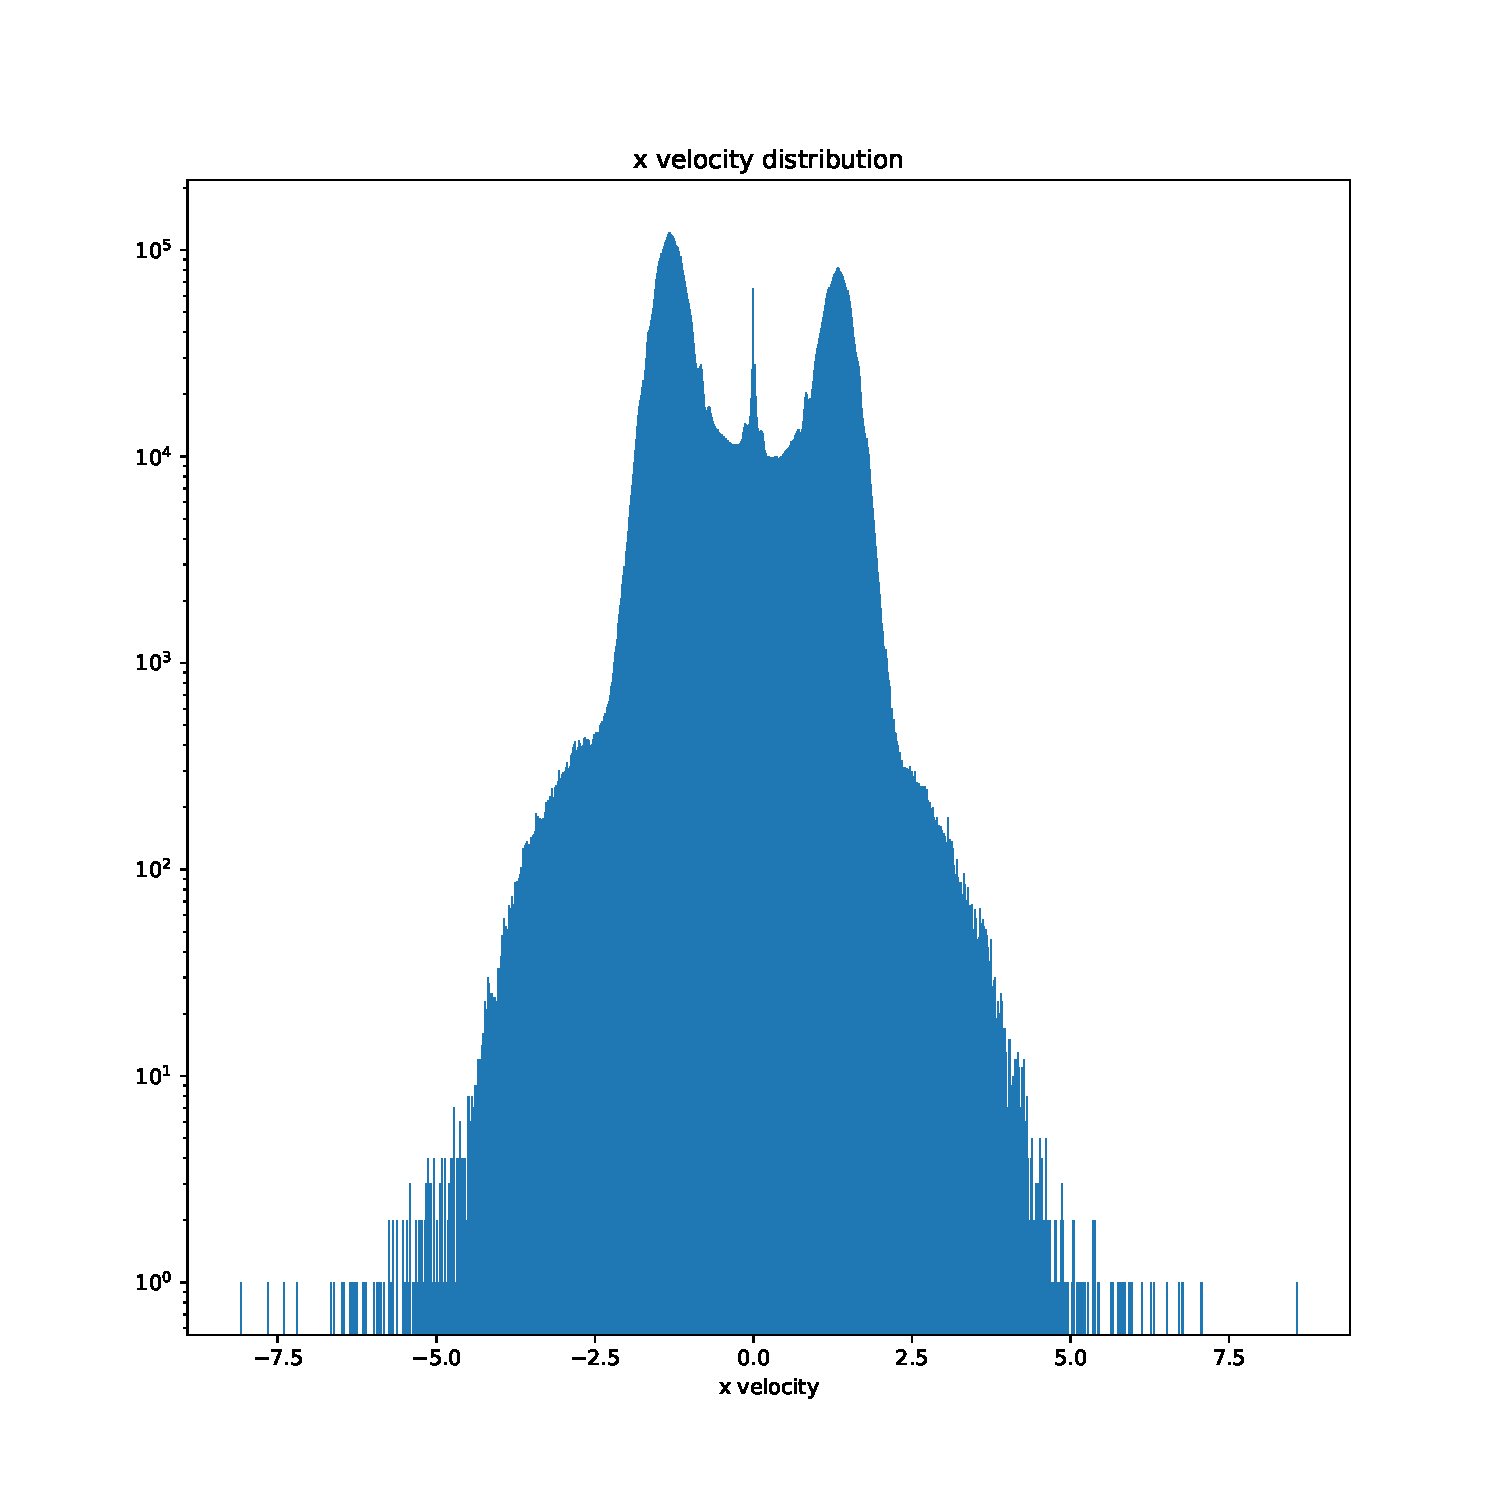
\includegraphics[ width=0.4\textwidth]{fig/hist_vx/save_trainf10_pro_RealData_hist_vx}
\captionsetup{width=0.9\linewidth}
\caption{Plot type (i). Real-life data distribution}
\label{fig:Vx_Real_i}
\end{minipage}
\begin{minipage}[c]{0.24\linewidth}
\centering
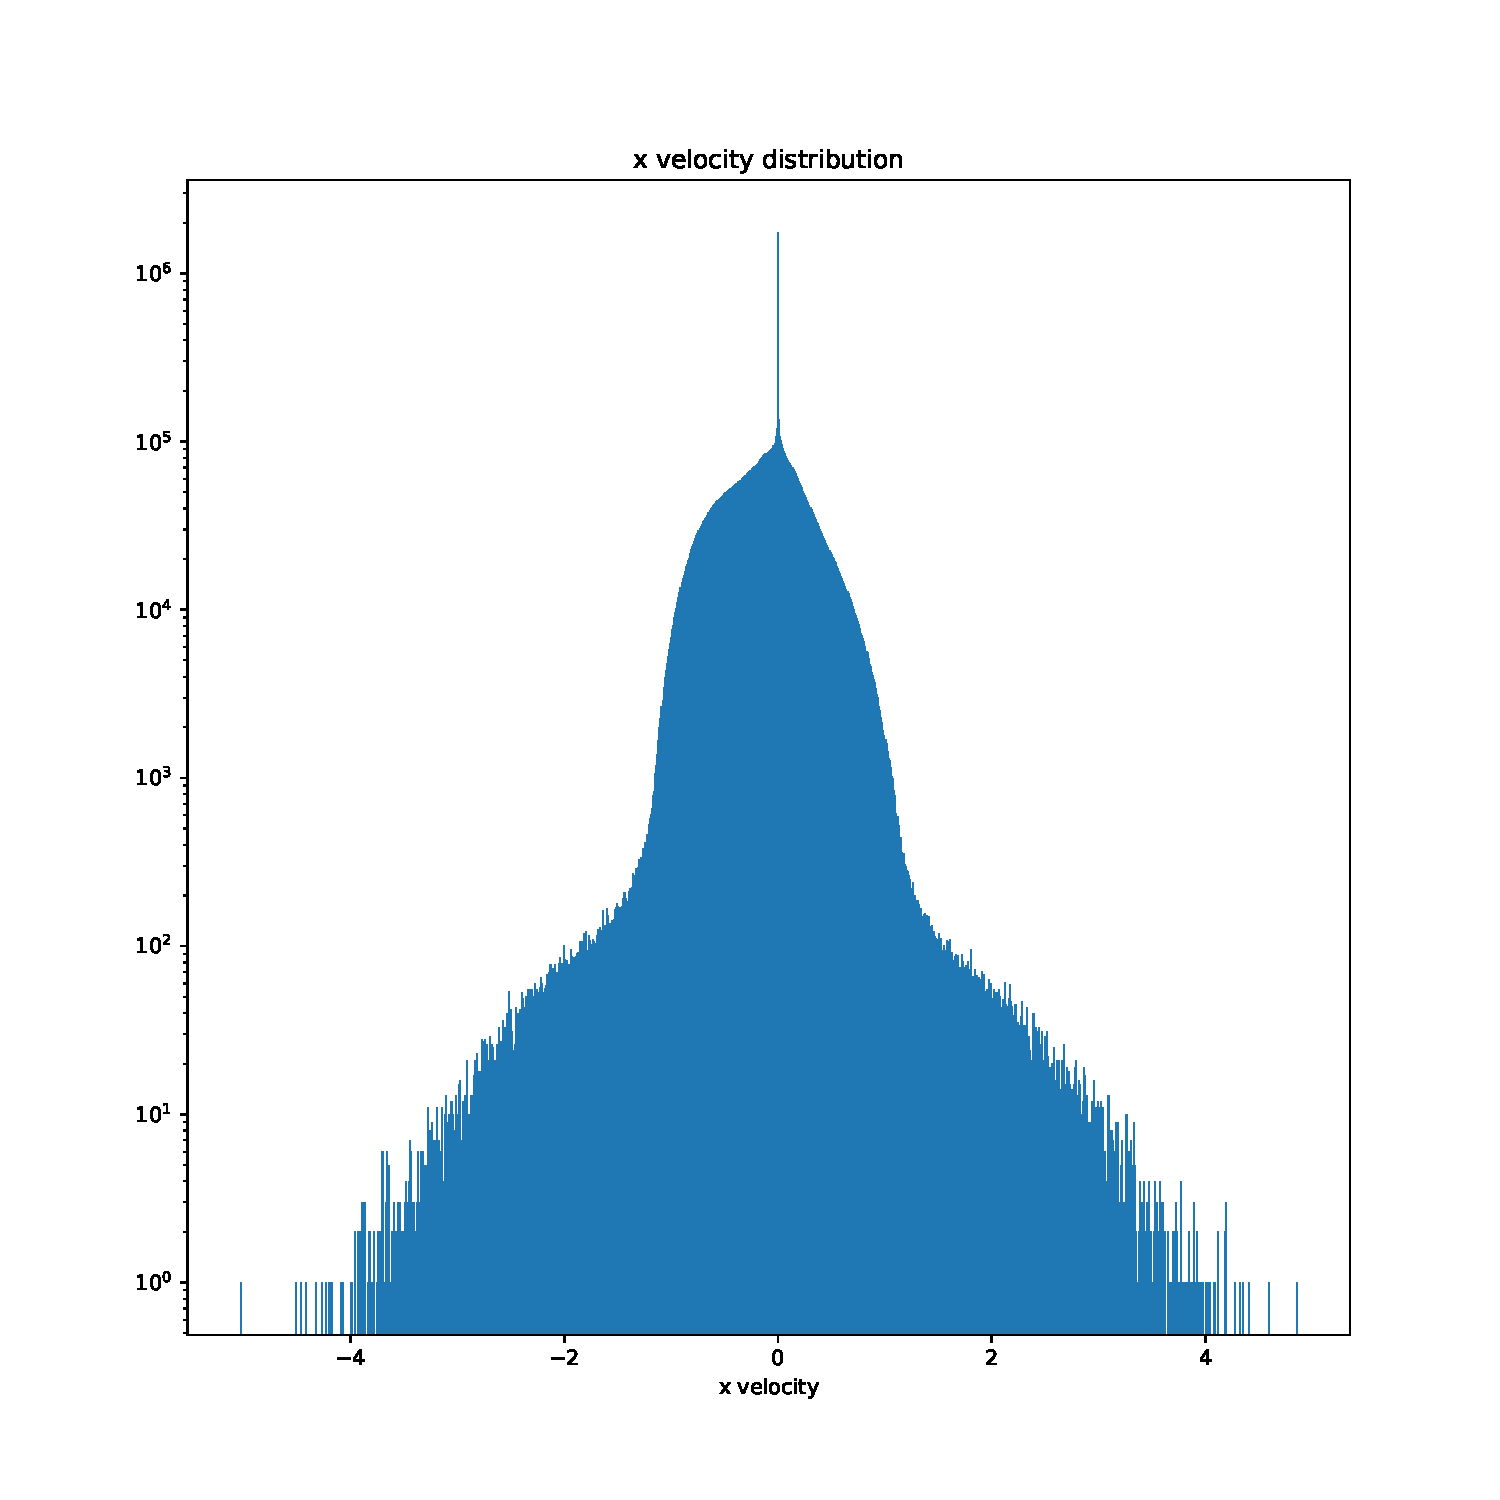
\includegraphics[ width=0.99\textwidth]{fig/hist_vx/save_trainf10_pro_simD2Q9_hist_vx}
\captionsetup{width=0.9\linewidth}
\caption{\\Plot type (i). \\Simulated dynamic using D2Q9}
\label{fig:Vx_SimD2Q9}
\end{minipage}
\begin{minipage}[c]{0.24\linewidth}
\centering
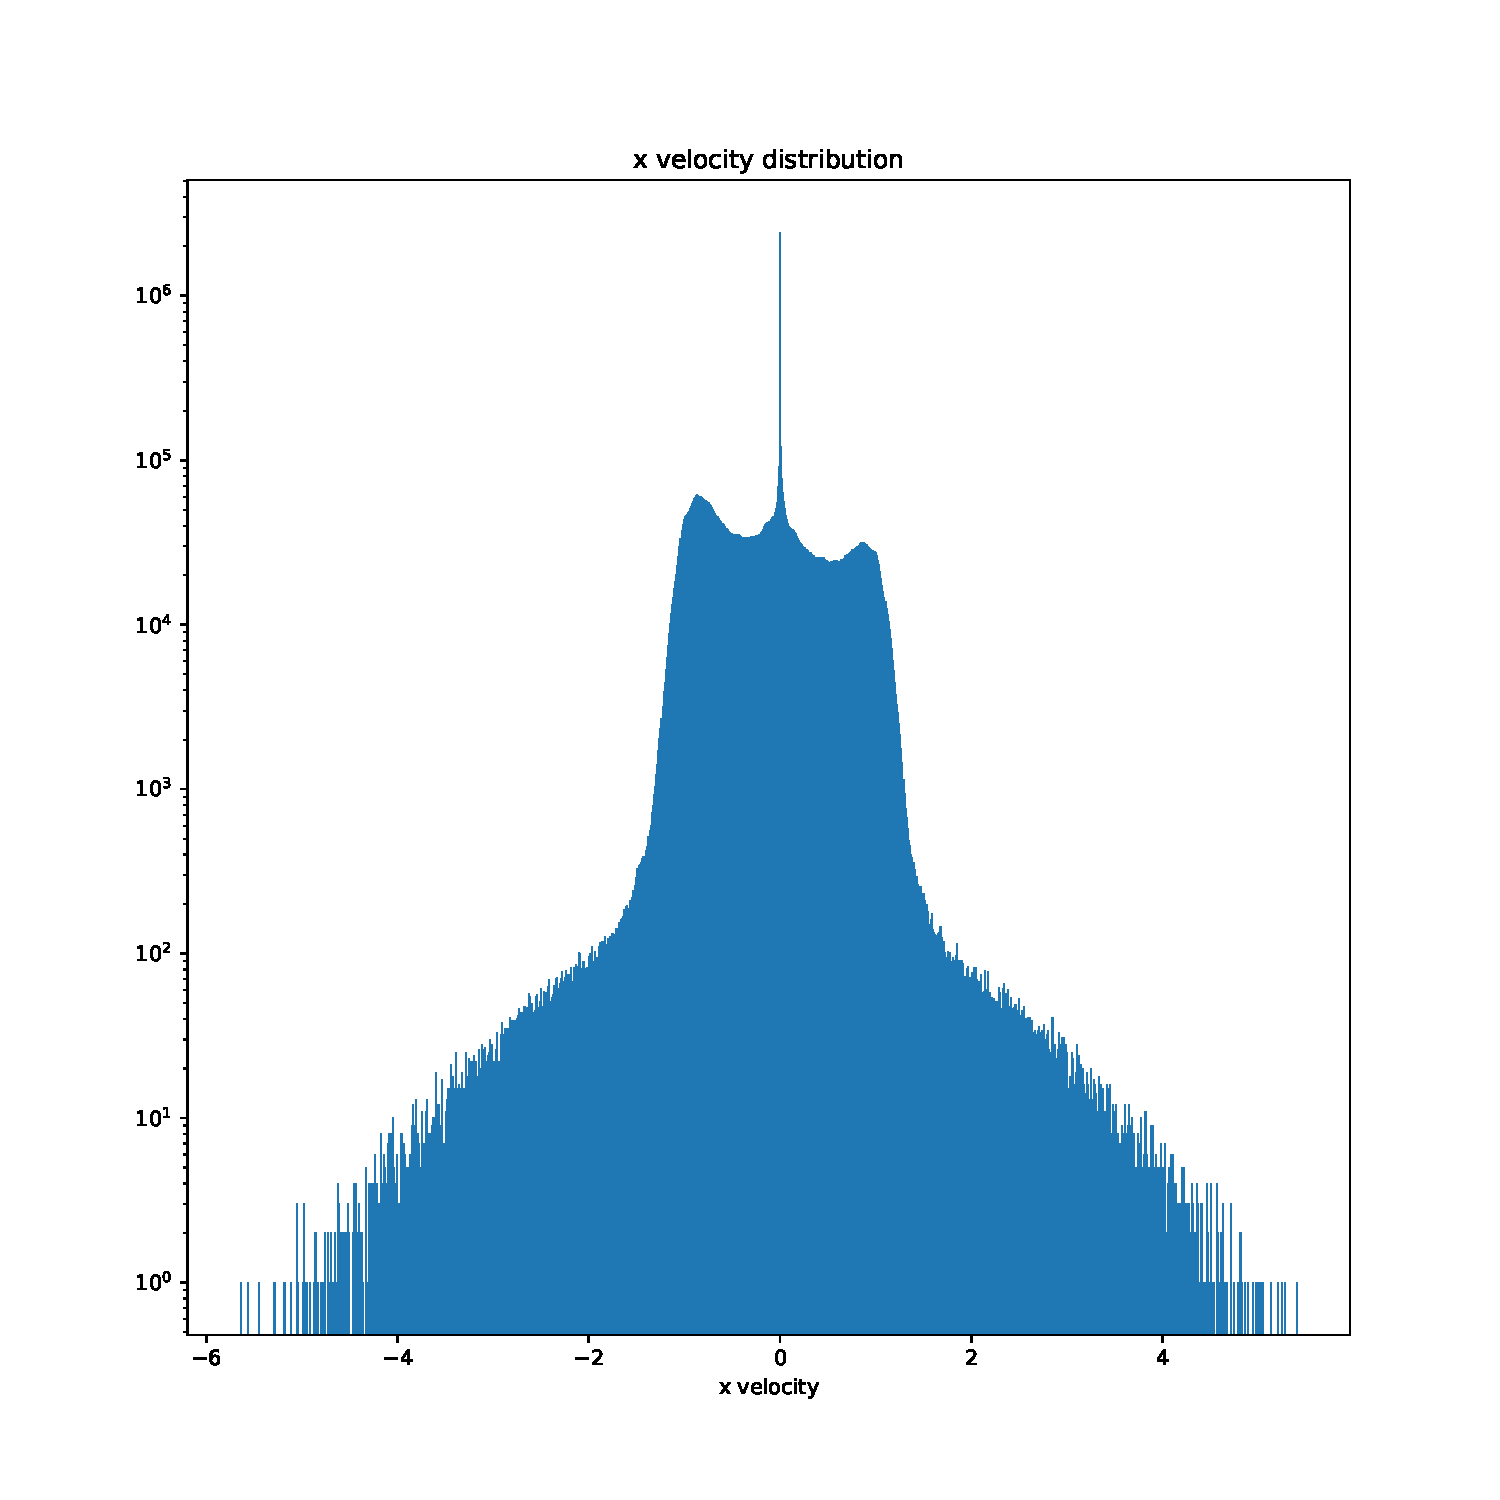
\includegraphics[ width=0.99\textwidth]{fig/hist_vx/save_trainf10_pro_simD2Q9Q9_hist_vx}
\captionsetup{width=0.9\linewidth}
\caption{\\Plot type (i). \\Simulated dynamic using D2Q9Q9}
\label{fig:Vx_SimD2Q9Q9}
\end{minipage}
\begin{minipage}[c]{0.24\linewidth}
\centering
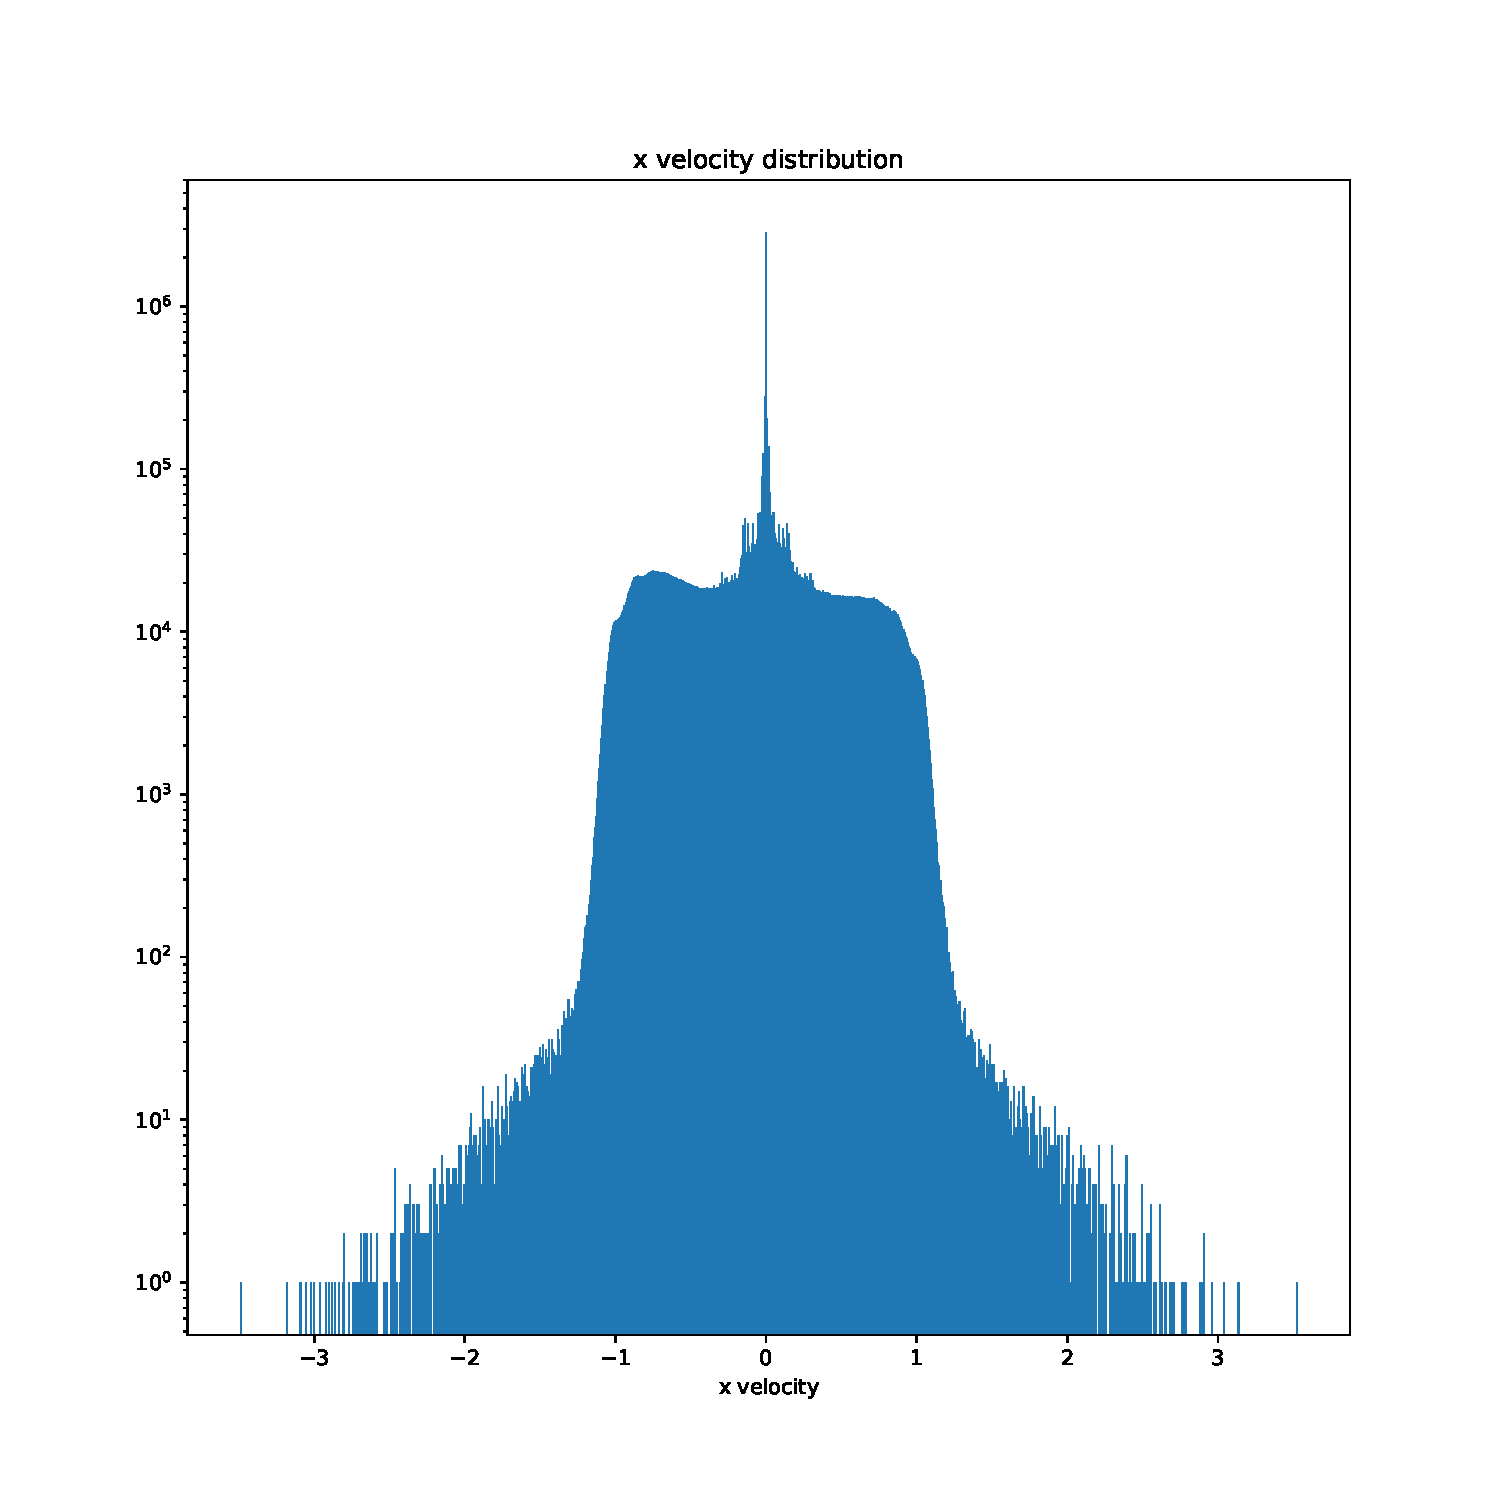
\includegraphics[ width=0.99\textwidth]{fig/hist_vx/save_trainf10_pro_simTD2Q9_hist_vx}
\captionsetup{width=0.9\linewidth}
\caption{\\Plot type (i). \\Simulated dynamic using TD2Q9}
\label{fig:Vx_SimTD2Q9}
\end{minipage}
\begin{minipage}[c]{0.24\linewidth}
\centering
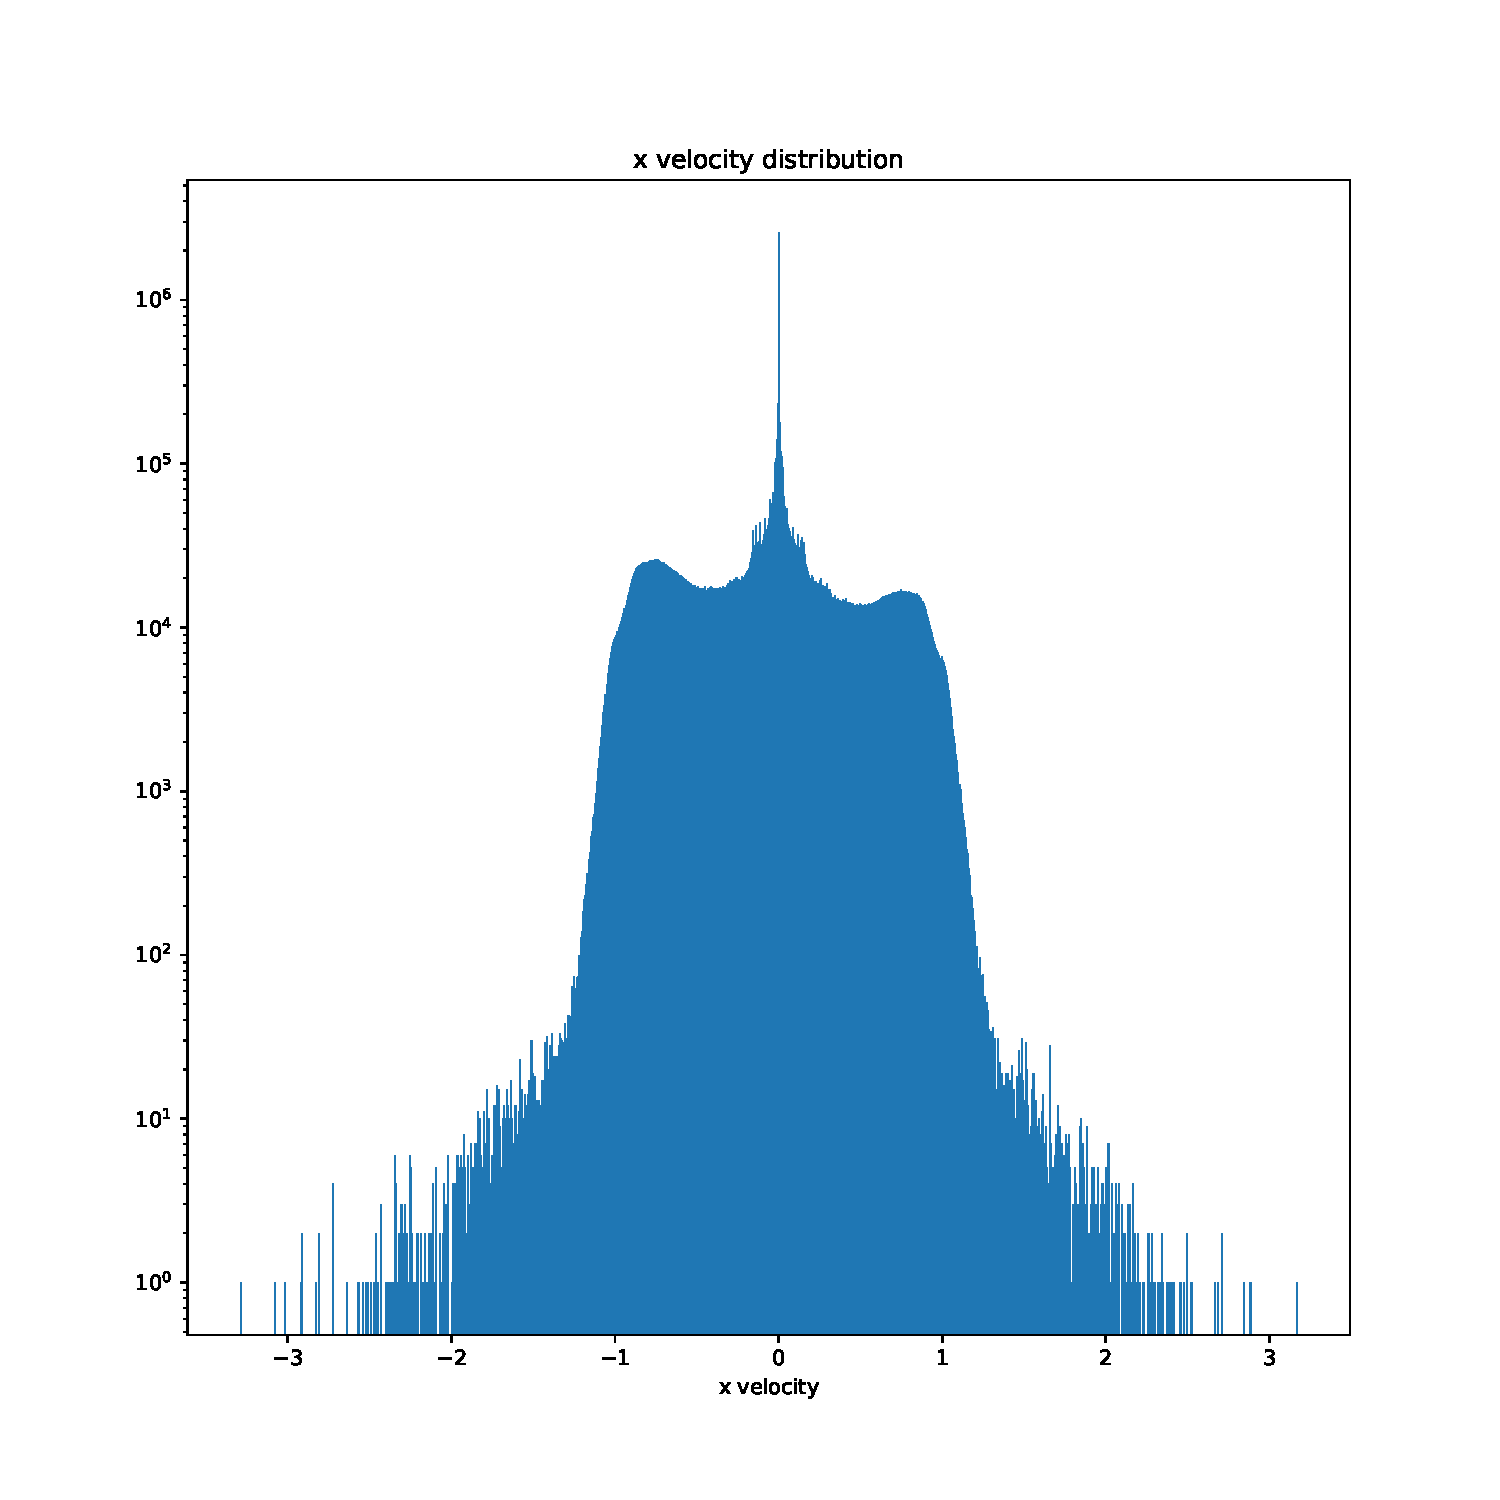
\includegraphics[ width=0.99\textwidth]{fig/hist_vx/save_trainf10_pro_simTD2Q9Q9_hist_vx}
\captionsetup{width=0.9\linewidth}
\caption{\\Plot type (i). \\Simulated dynamic using TD2Q9Q9}
\label{fig:Vx_SimTD2Q9Q9}
\end{minipage}
\end{figure}


% --- --- --- --- --- --- --- --- --- --- --- --- --- --- --- --- --- --- --- --- --- --- --- --- --- --- --- --- --- --- --- --- --- ---


\begin{figure}[ht]
\begin{minipage}[c]{1\linewidth}
\centering
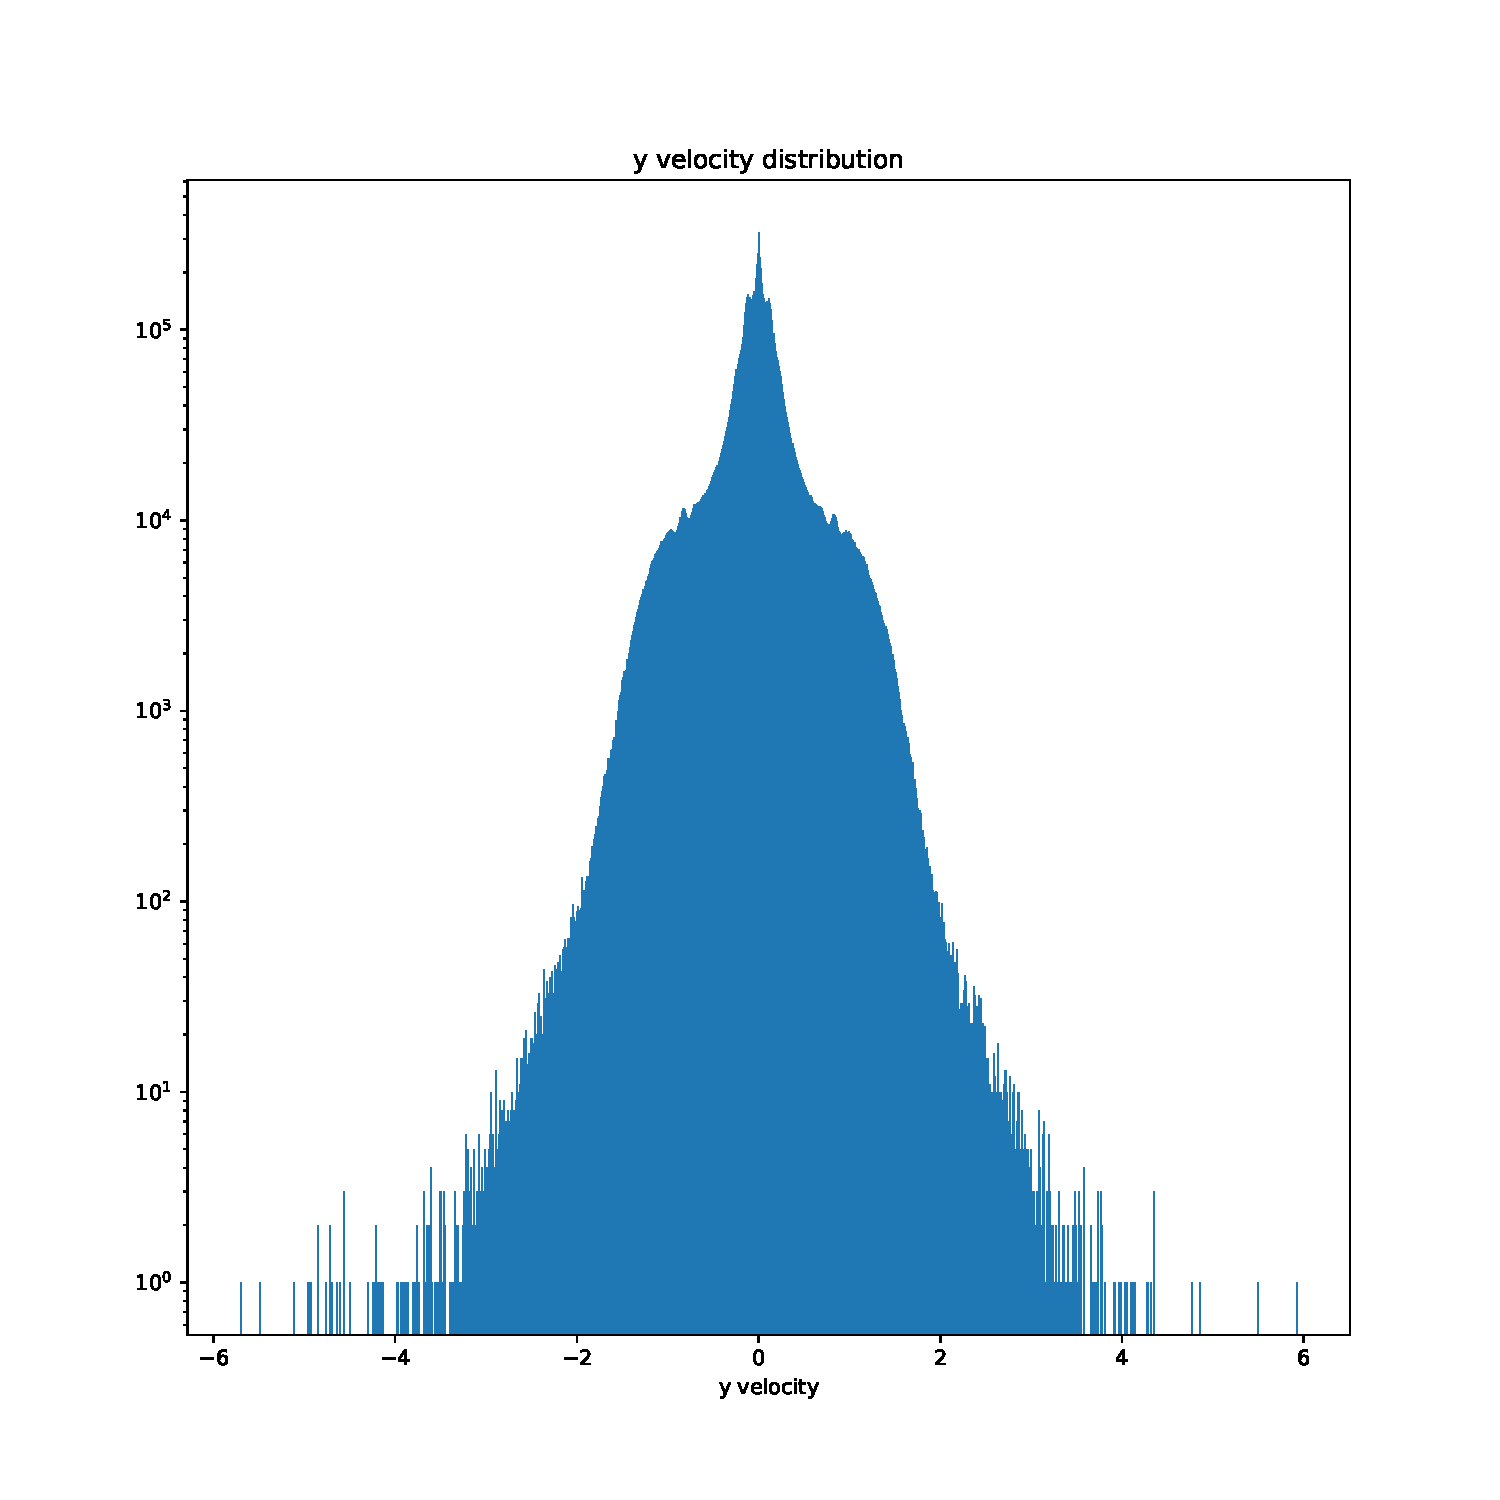
\includegraphics[ width=0.4\textwidth]{fig/hist_vy/save_trainf10_pro_RealData_hist_vy}
\captionsetup{width=0.9\linewidth}
\caption{Plot type (ii). Real-life data distribution}
\label{fig:Vy_Real_ii}
\end{minipage}
\begin{minipage}[c]{0.24\linewidth}
\centering
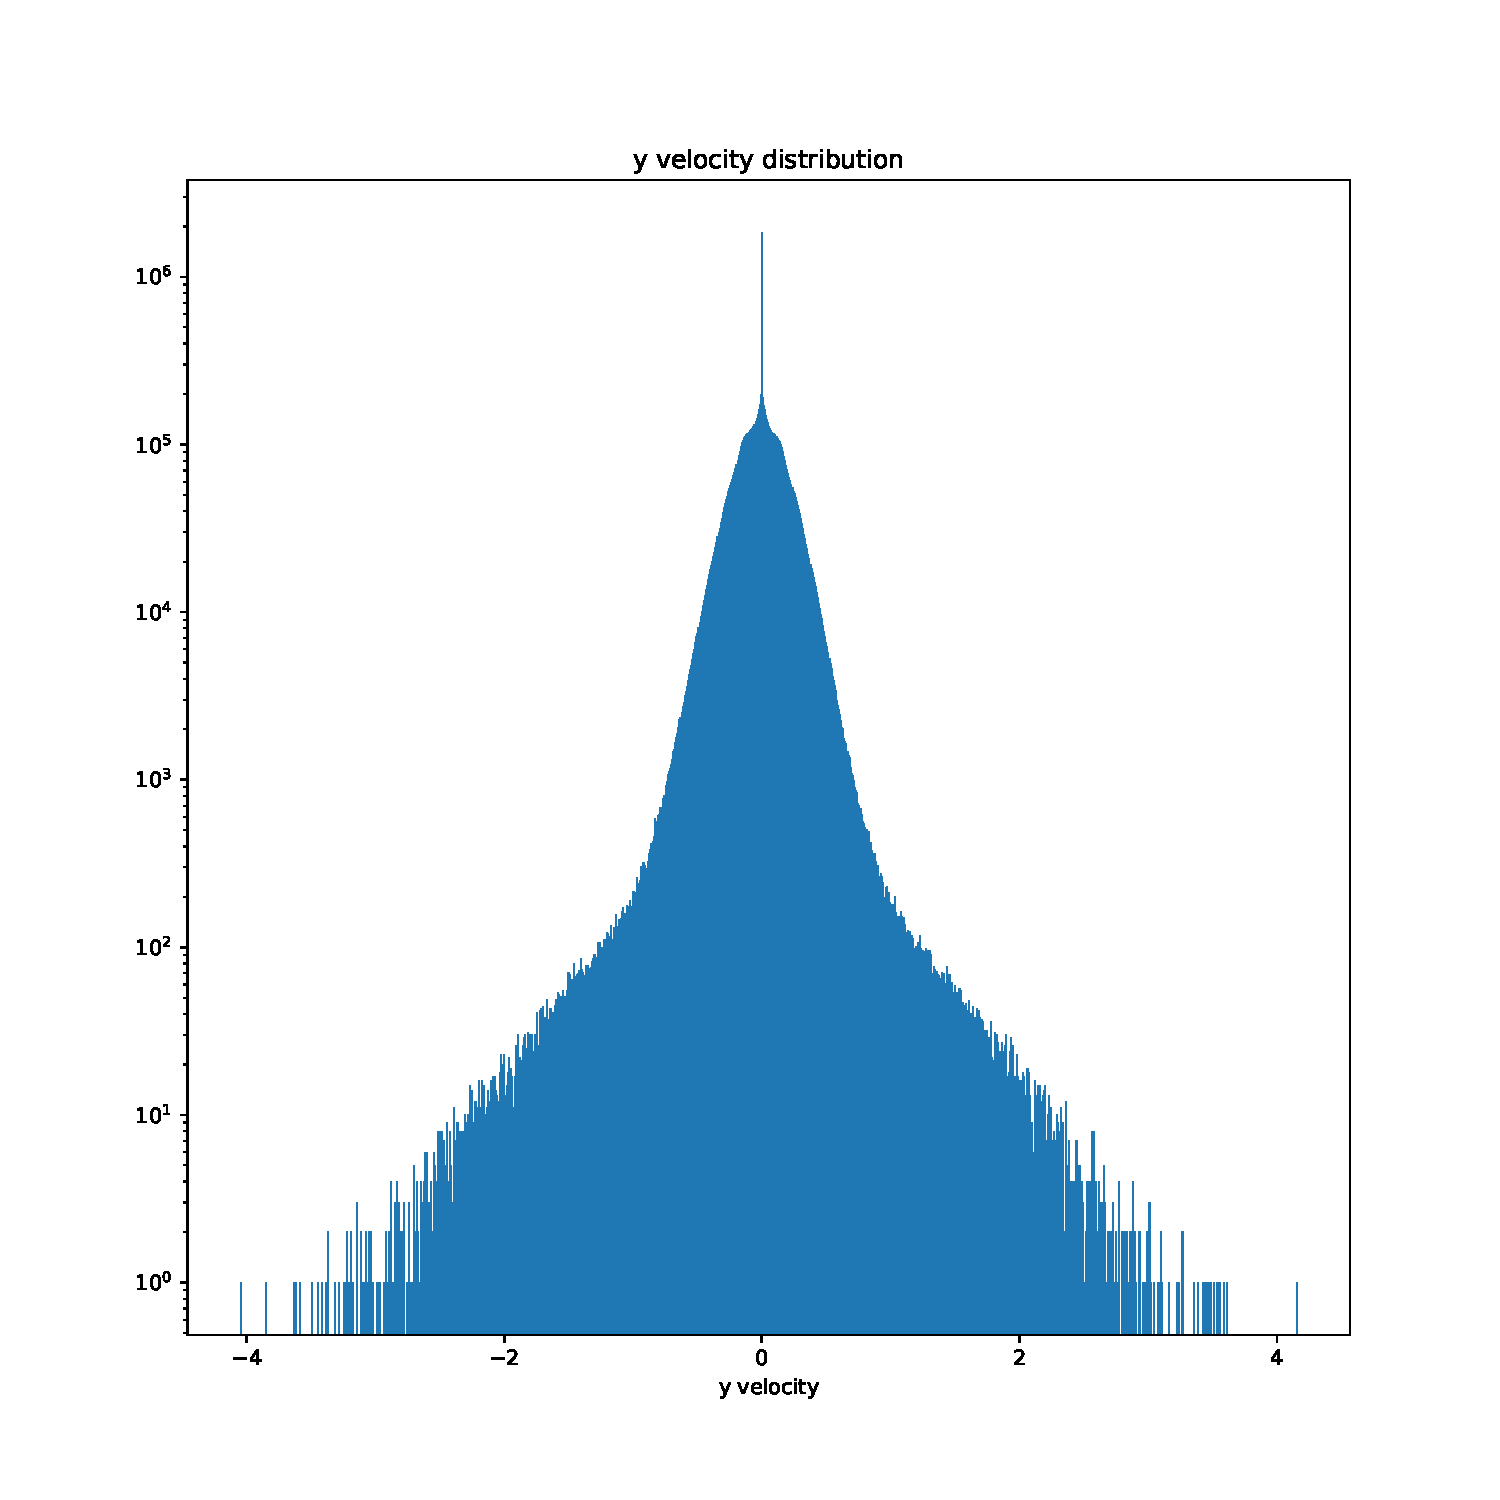
\includegraphics[ width=0.99\textwidth]{fig/hist_vy/save_trainf10_pro_simD2Q9_hist_vy}
\captionsetup{width=0.9\linewidth}
\caption{\\Plot type (ii). \\Simulated dynamic using D2Q9}
\label{fig:Vy_SimD2Q9}
\end{minipage}
\begin{minipage}[c]{0.24\linewidth}
\centering
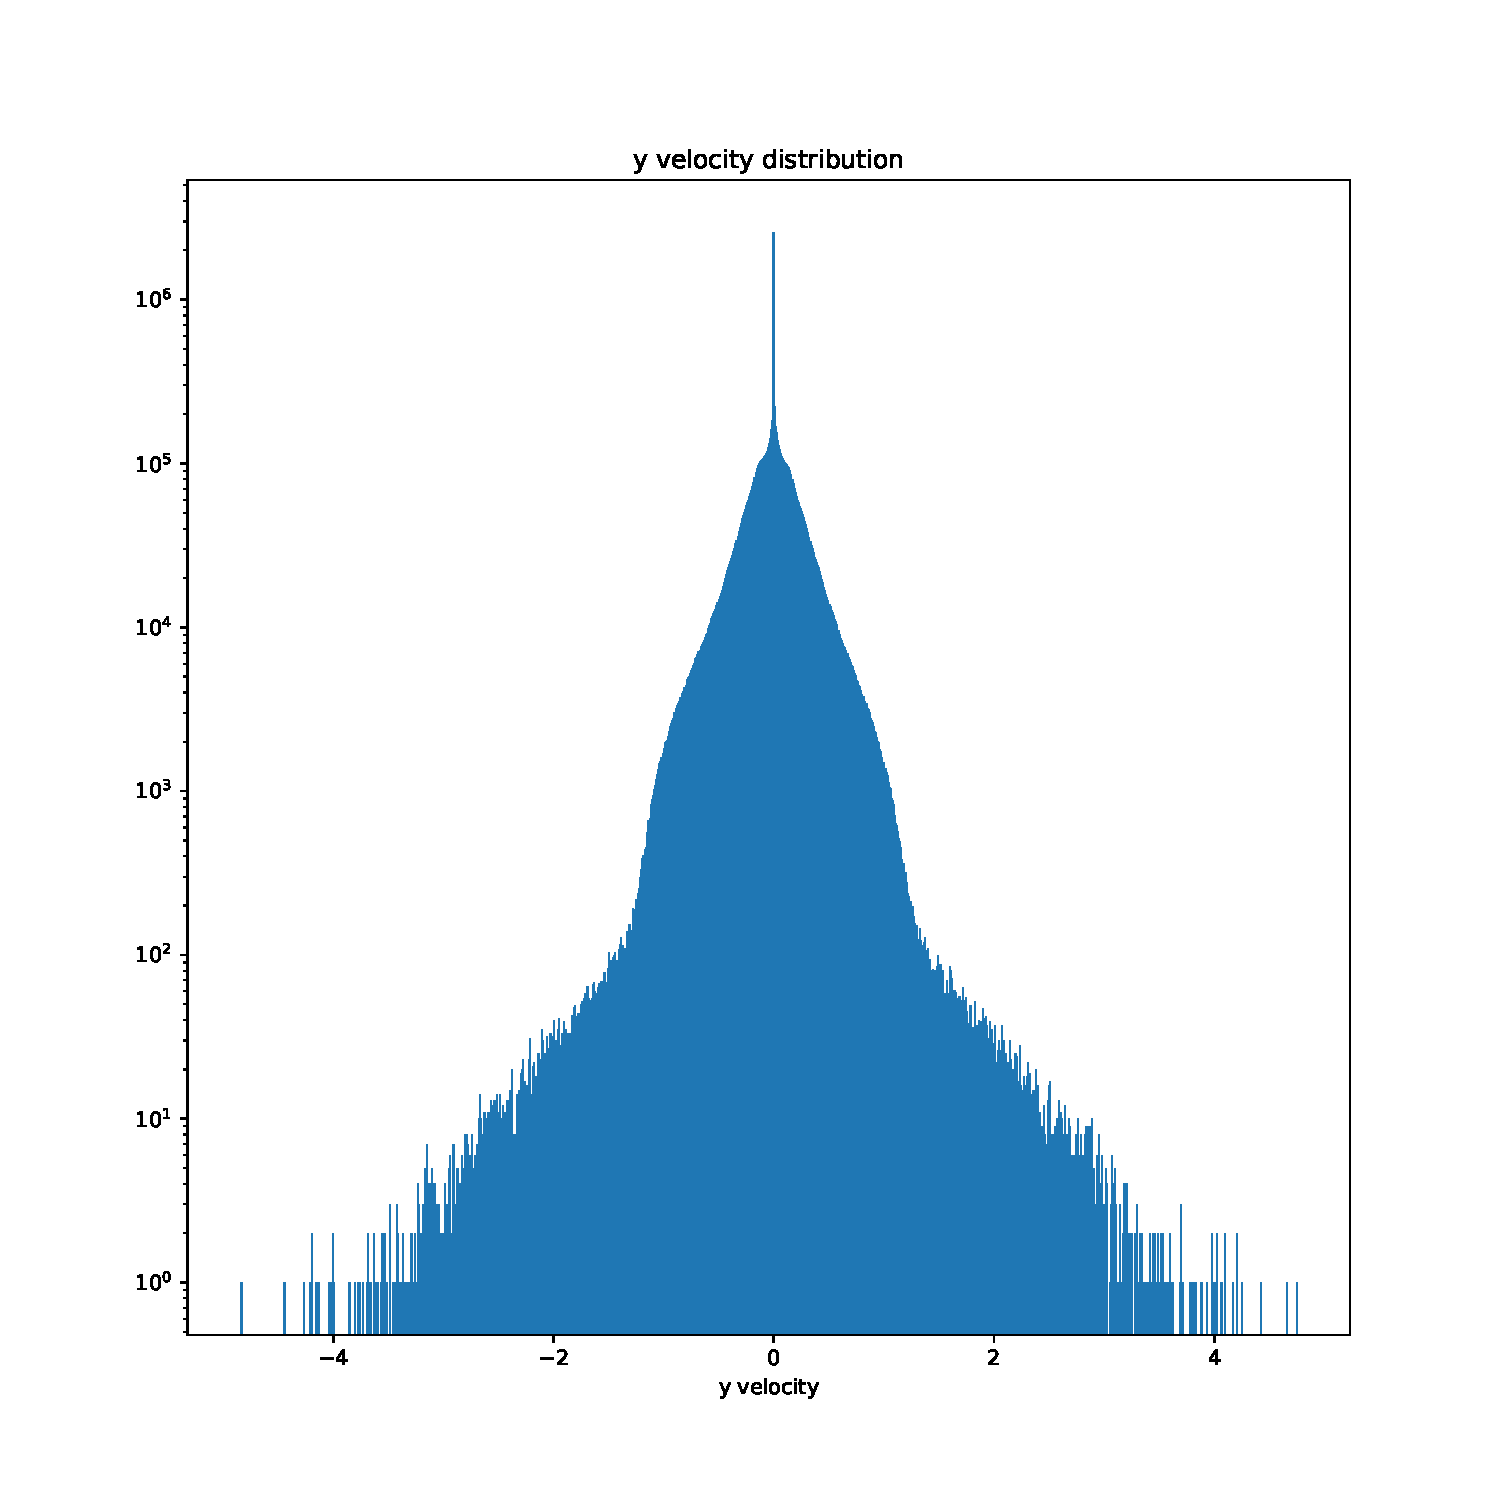
\includegraphics[ width=0.99\textwidth]{fig/hist_vy/save_trainf10_pro_simD2Q9Q9_hist_vy}
\captionsetup{width=0.9\linewidth}
\caption{\\Plot type (ii). \\Simulated dynamic using D2Q9Q9}
\label{fig:Vy_SimD2Q9Q9}
\end{minipage}
\begin{minipage}[c]{0.24\linewidth}
\centering
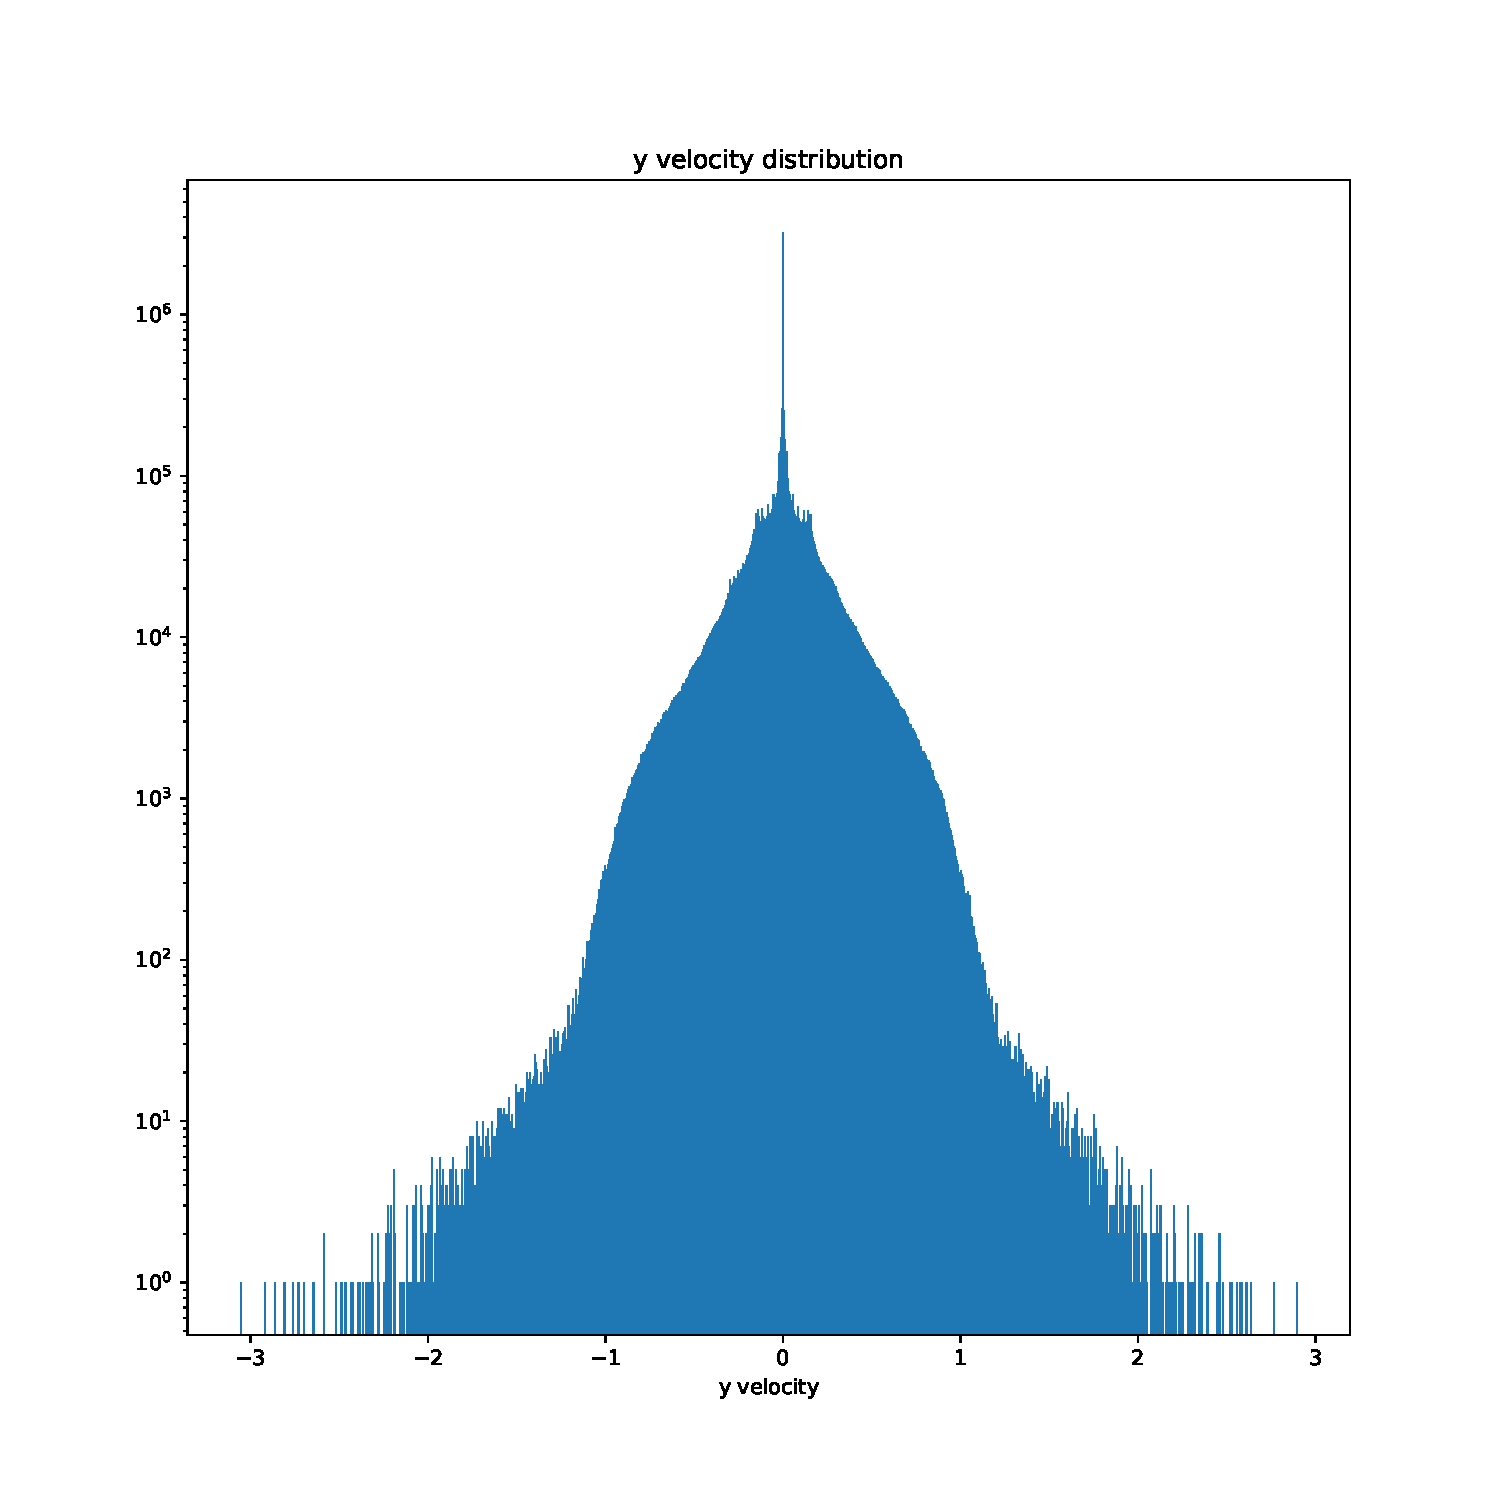
\includegraphics[ width=0.99\textwidth]{fig/hist_vy/save_trainf10_pro_simTD2Q9_hist_vy}
\captionsetup{width=0.9\linewidth}
\caption{\\Plot type (ii). \\Simulated dynamic using TD2Q9}
\label{fig:Vy_SimTD2Q9}
\end{minipage}
\begin{minipage}[c]{0.24\linewidth}
\centering
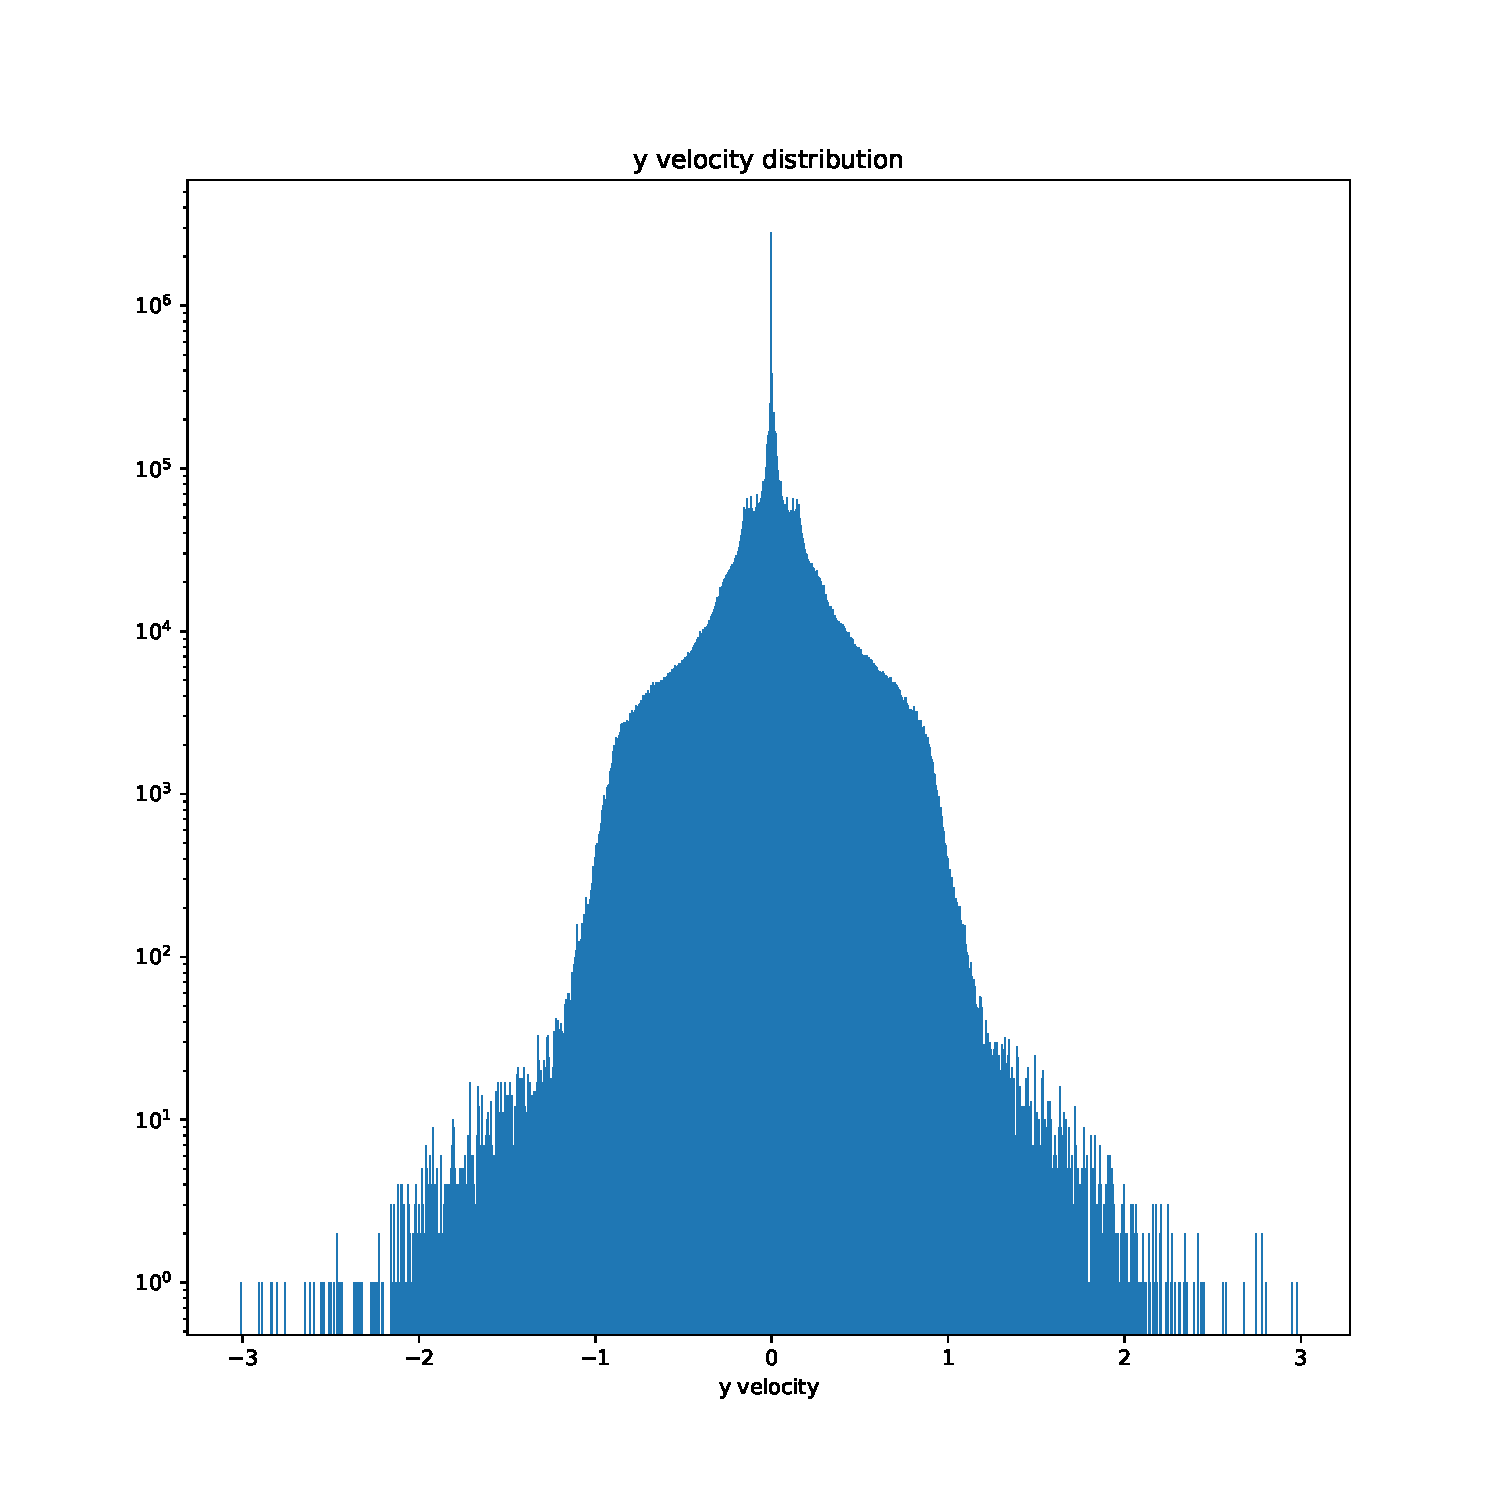
\includegraphics[ width=0.99\textwidth]{fig/hist_vy/save_trainf10_pro_simTD2Q9Q9_hist_vy}
\captionsetup{width=0.9\linewidth}
\caption{\\Plot type (ii). \\Simulated dynamic using TD2Q9Q9}
\label{fig:Vy_SimTD2Q9Q9}
\end{minipage}
\end{figure}


% --- --- --- --- --- --- --- --- --- --- --- --- --- --- --- --- --- --- --- --- --- --- --- --- --- --- --- --- --- --- --- --- --- ---


\begin{figure}[ht]
\begin{minipage}[c]{1\linewidth}
\centering
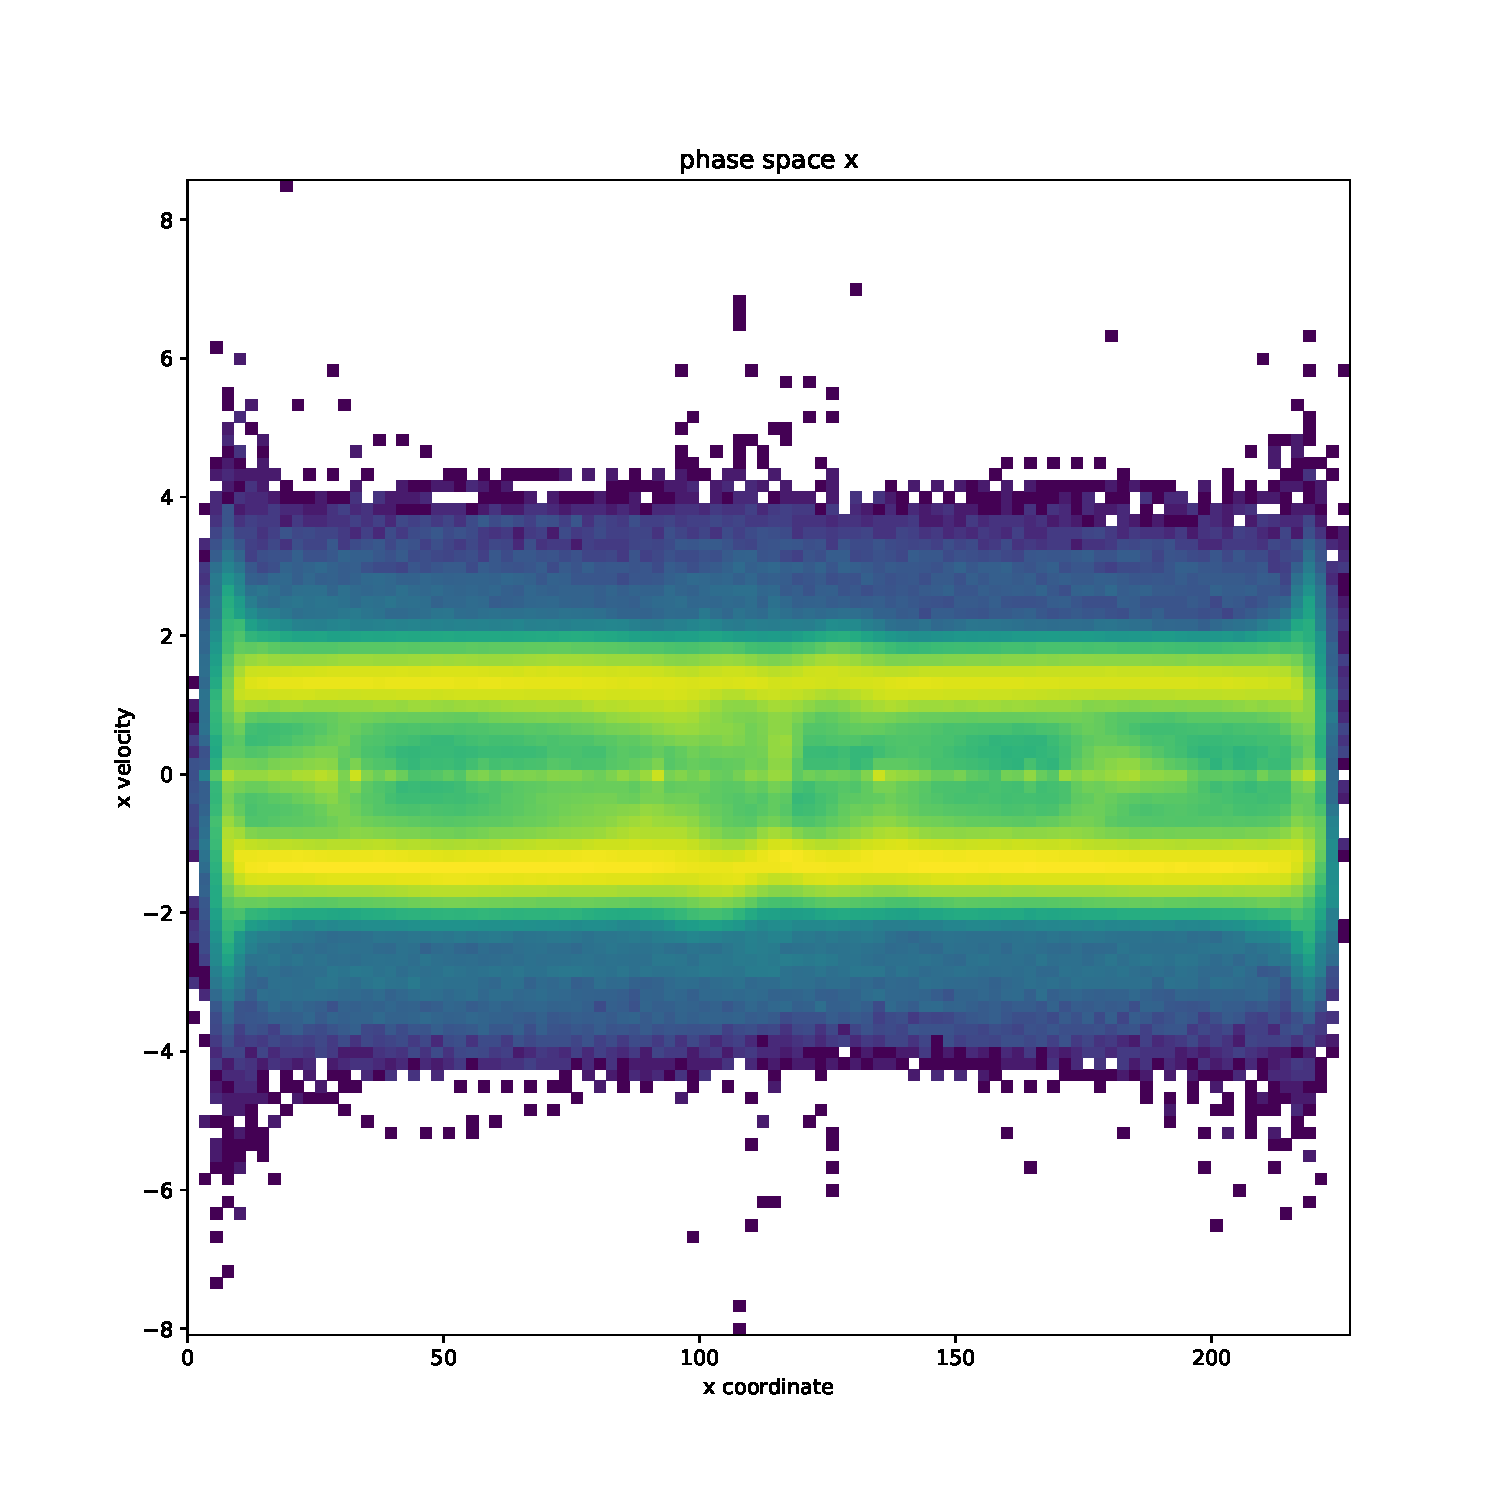
\includegraphics[ width=0.4\textwidth]{fig/hist2d_xvx/save_trainf10_pro_RealData_hist2d_x_vx}
\captionsetup{width=0.9\linewidth}
\caption{Plot type (iii). Real-life data distribution}
\label{fig:xVx_Real_iii}
\end{minipage}
\begin{minipage}[c]{0.24\linewidth}
\centering
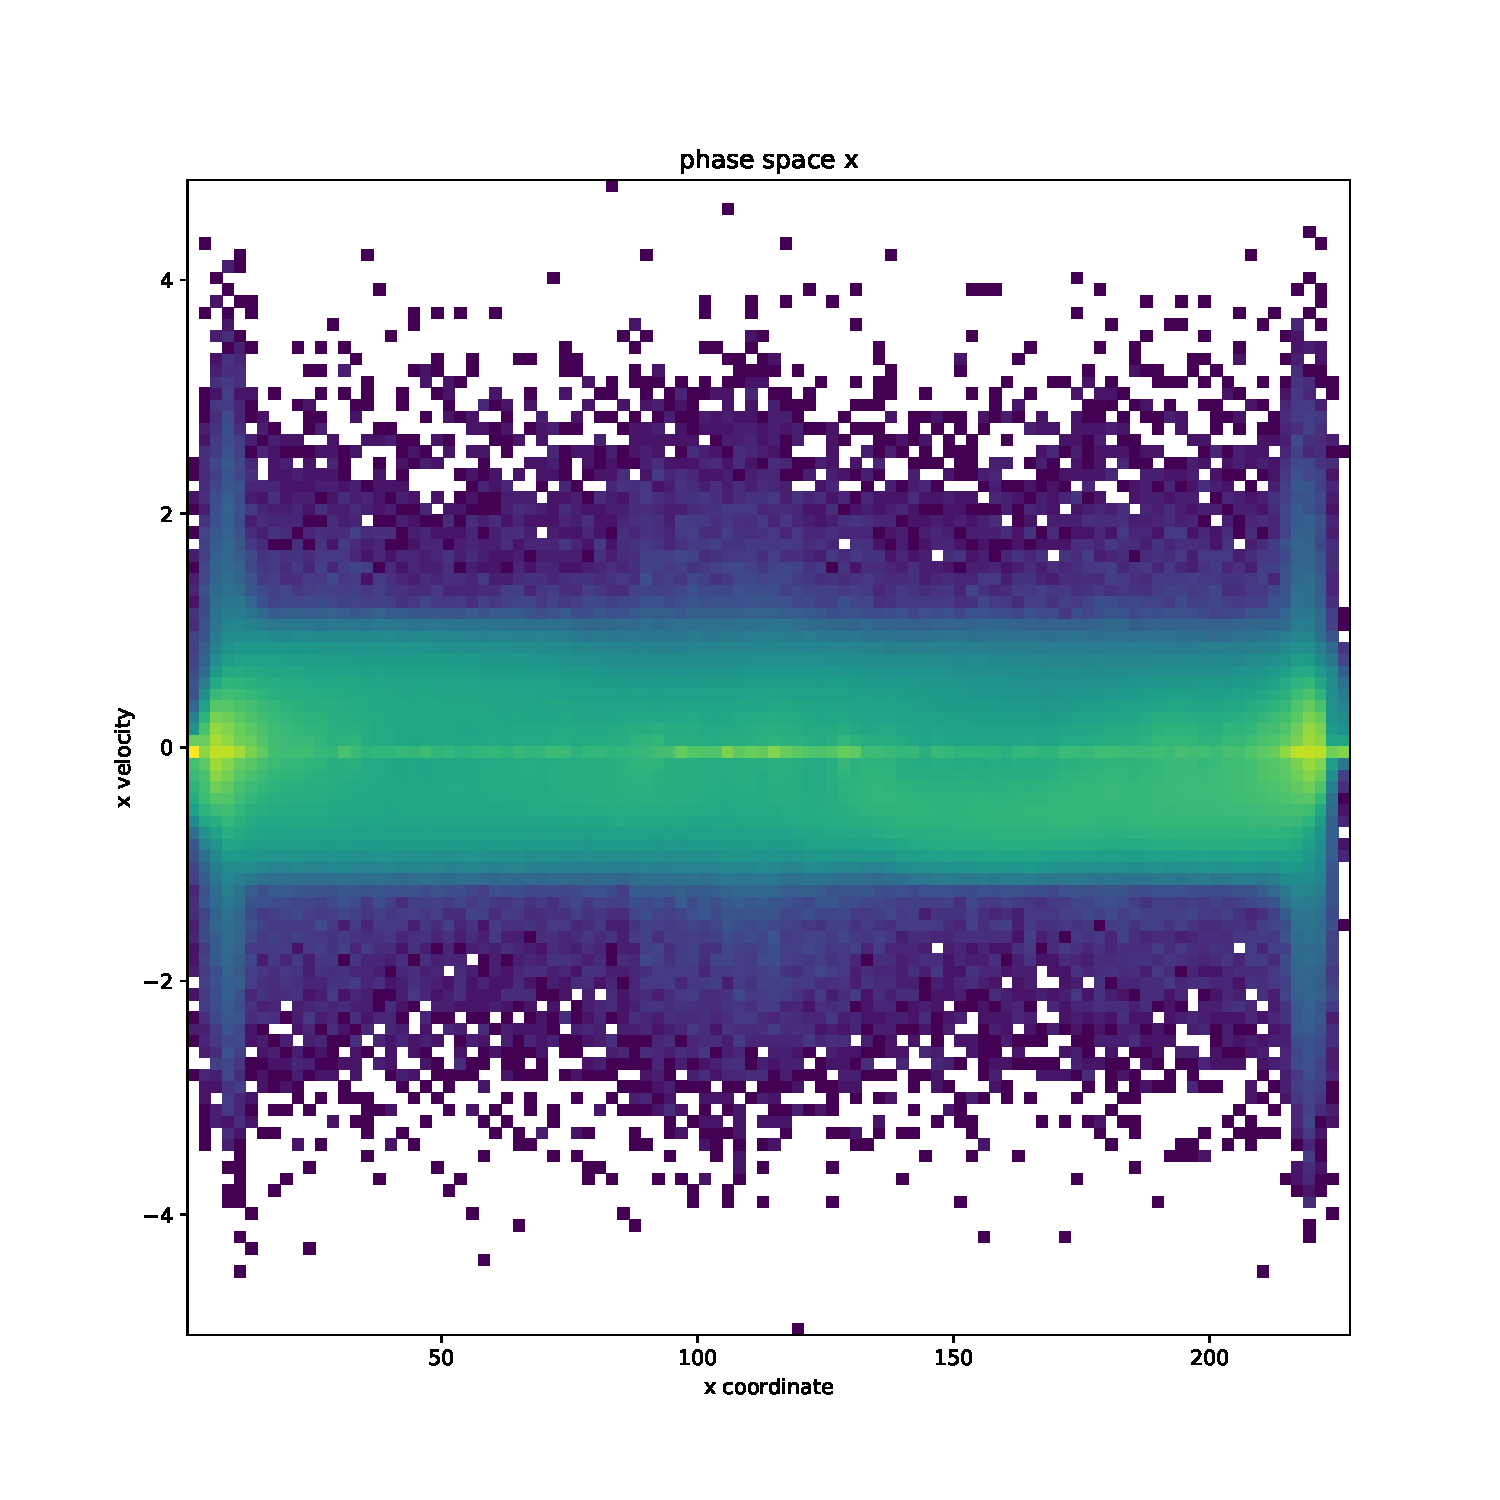
\includegraphics[ width=0.99\textwidth]{fig/hist2d_xvx/save_trainf10_pro_simD2Q9_hist2d_x_vx}
\captionsetup{width=0.9\linewidth}
\caption{\\Plot type (iii). \\Simulated dynamic using D2Q9}
\label{fig:xVx_SimD2Q9}
\end{minipage}
\begin{minipage}[c]{0.24\linewidth}
\centering
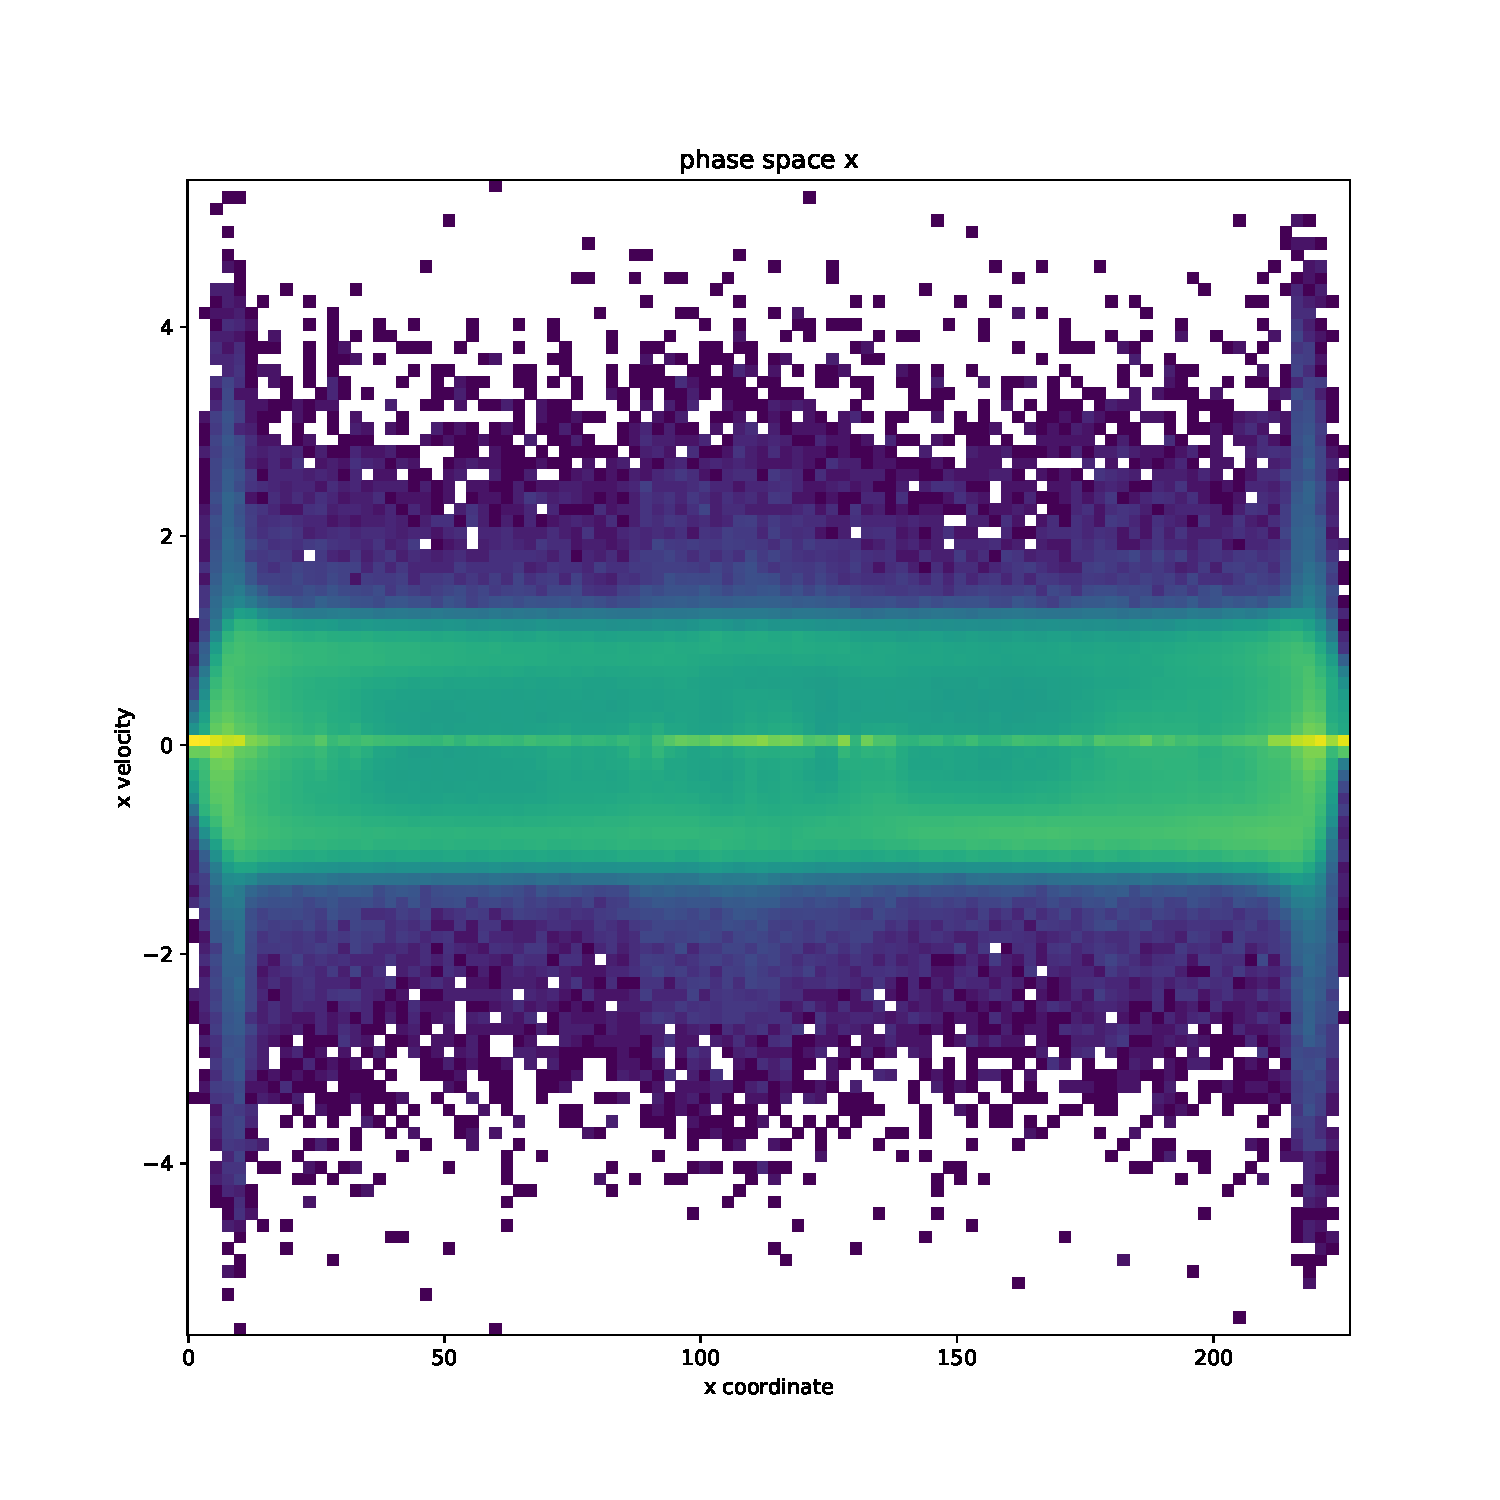
\includegraphics[ width=0.99\textwidth]{fig/hist2d_xvx/save_trainf10_pro_simD2Q9Q9_hist2d_x_vx}
\captionsetup{width=0.9\linewidth}
\caption{\\Plot type (iii). \\Simulated dynamic using D2Q9Q9}
\label{fig:xVx_SimD2Q9Q9}
\end{minipage}
\begin{minipage}[c]{0.24\linewidth}
\centering
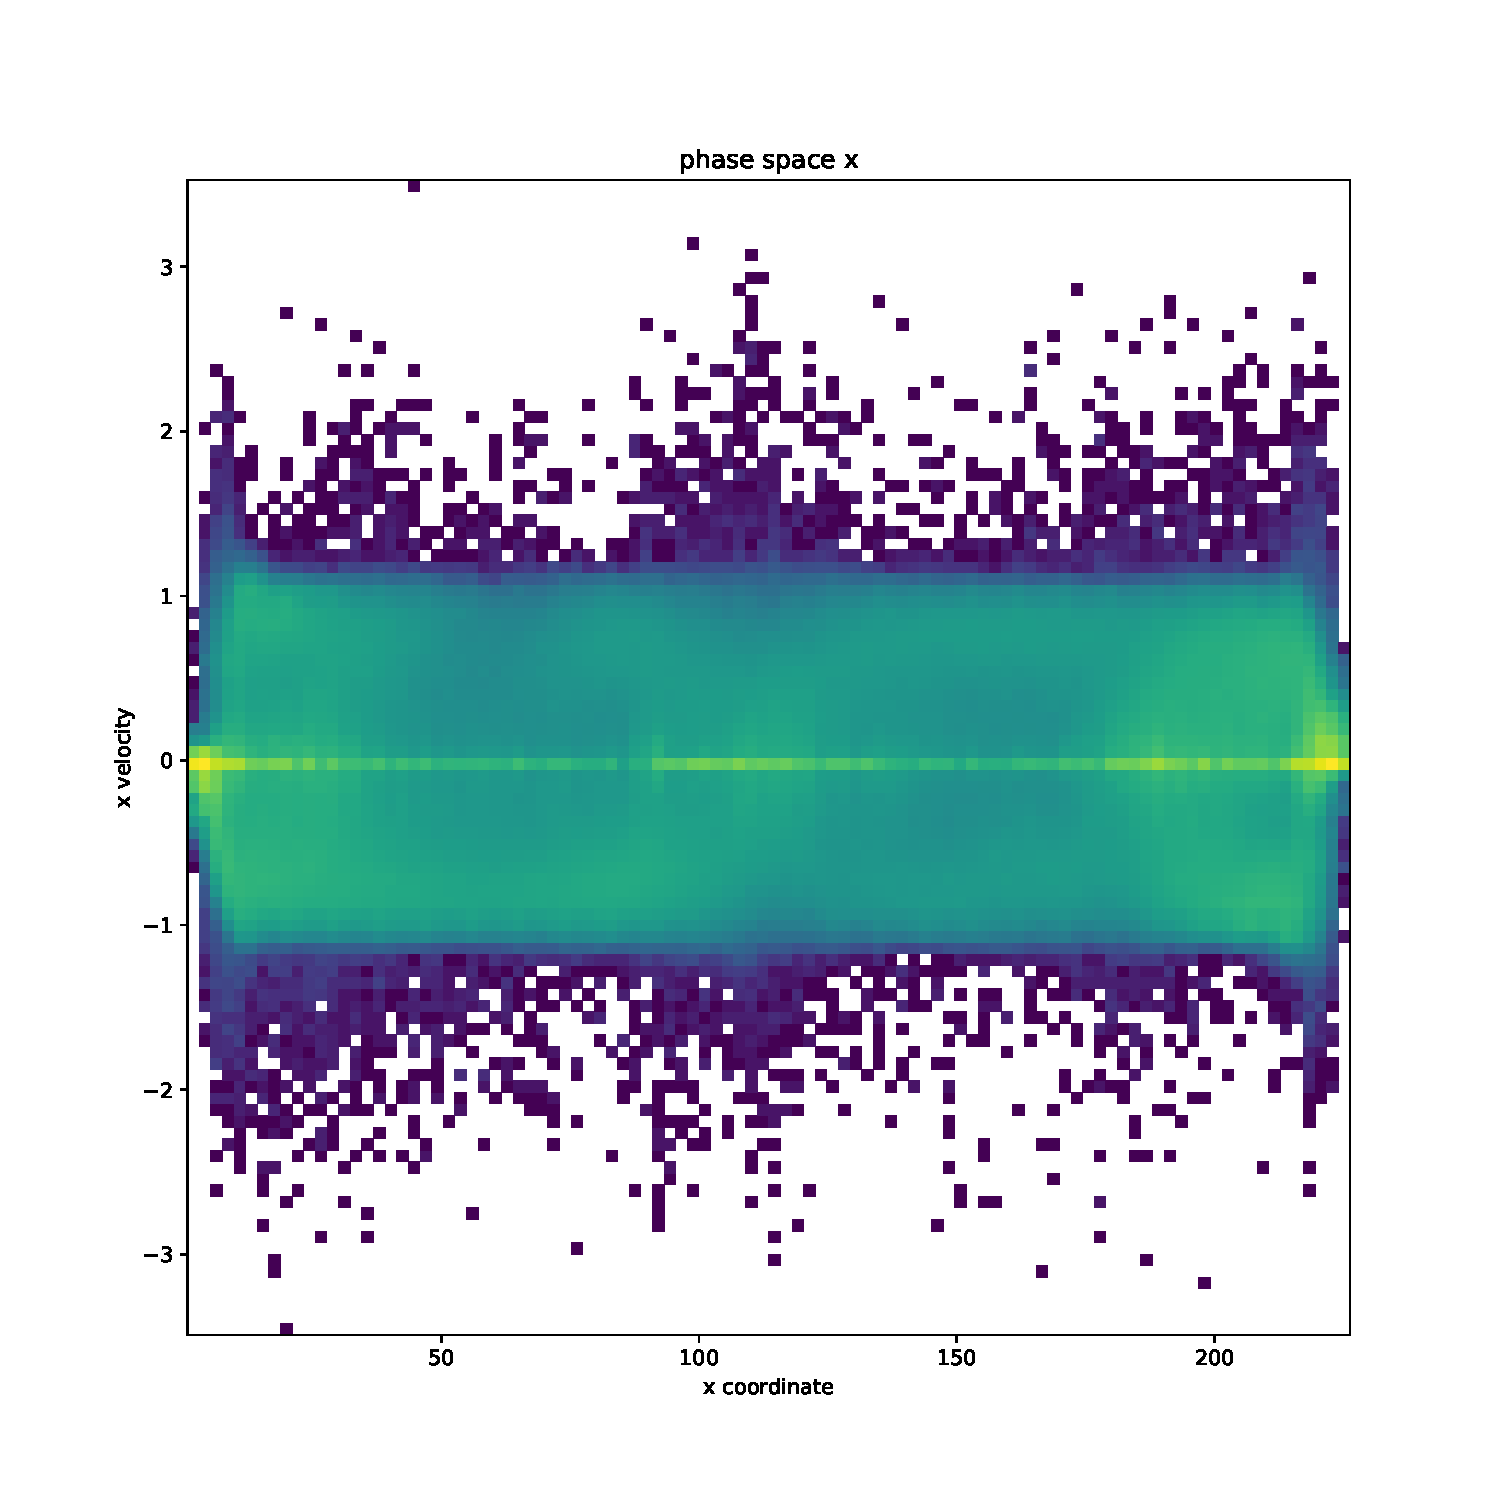
\includegraphics[ width=0.99\textwidth]{fig/hist2d_xvx/save_trainf10_pro_simTD2Q9_hist2d_x_vx}
\captionsetup{width=0.9\linewidth}
\caption{\\Plot type (iii). \\Simulated dynamic using TD2Q9}
\label{fig:xVx_SimTD2Q9}
\end{minipage}
\begin{minipage}[c]{0.24\linewidth}
\centering
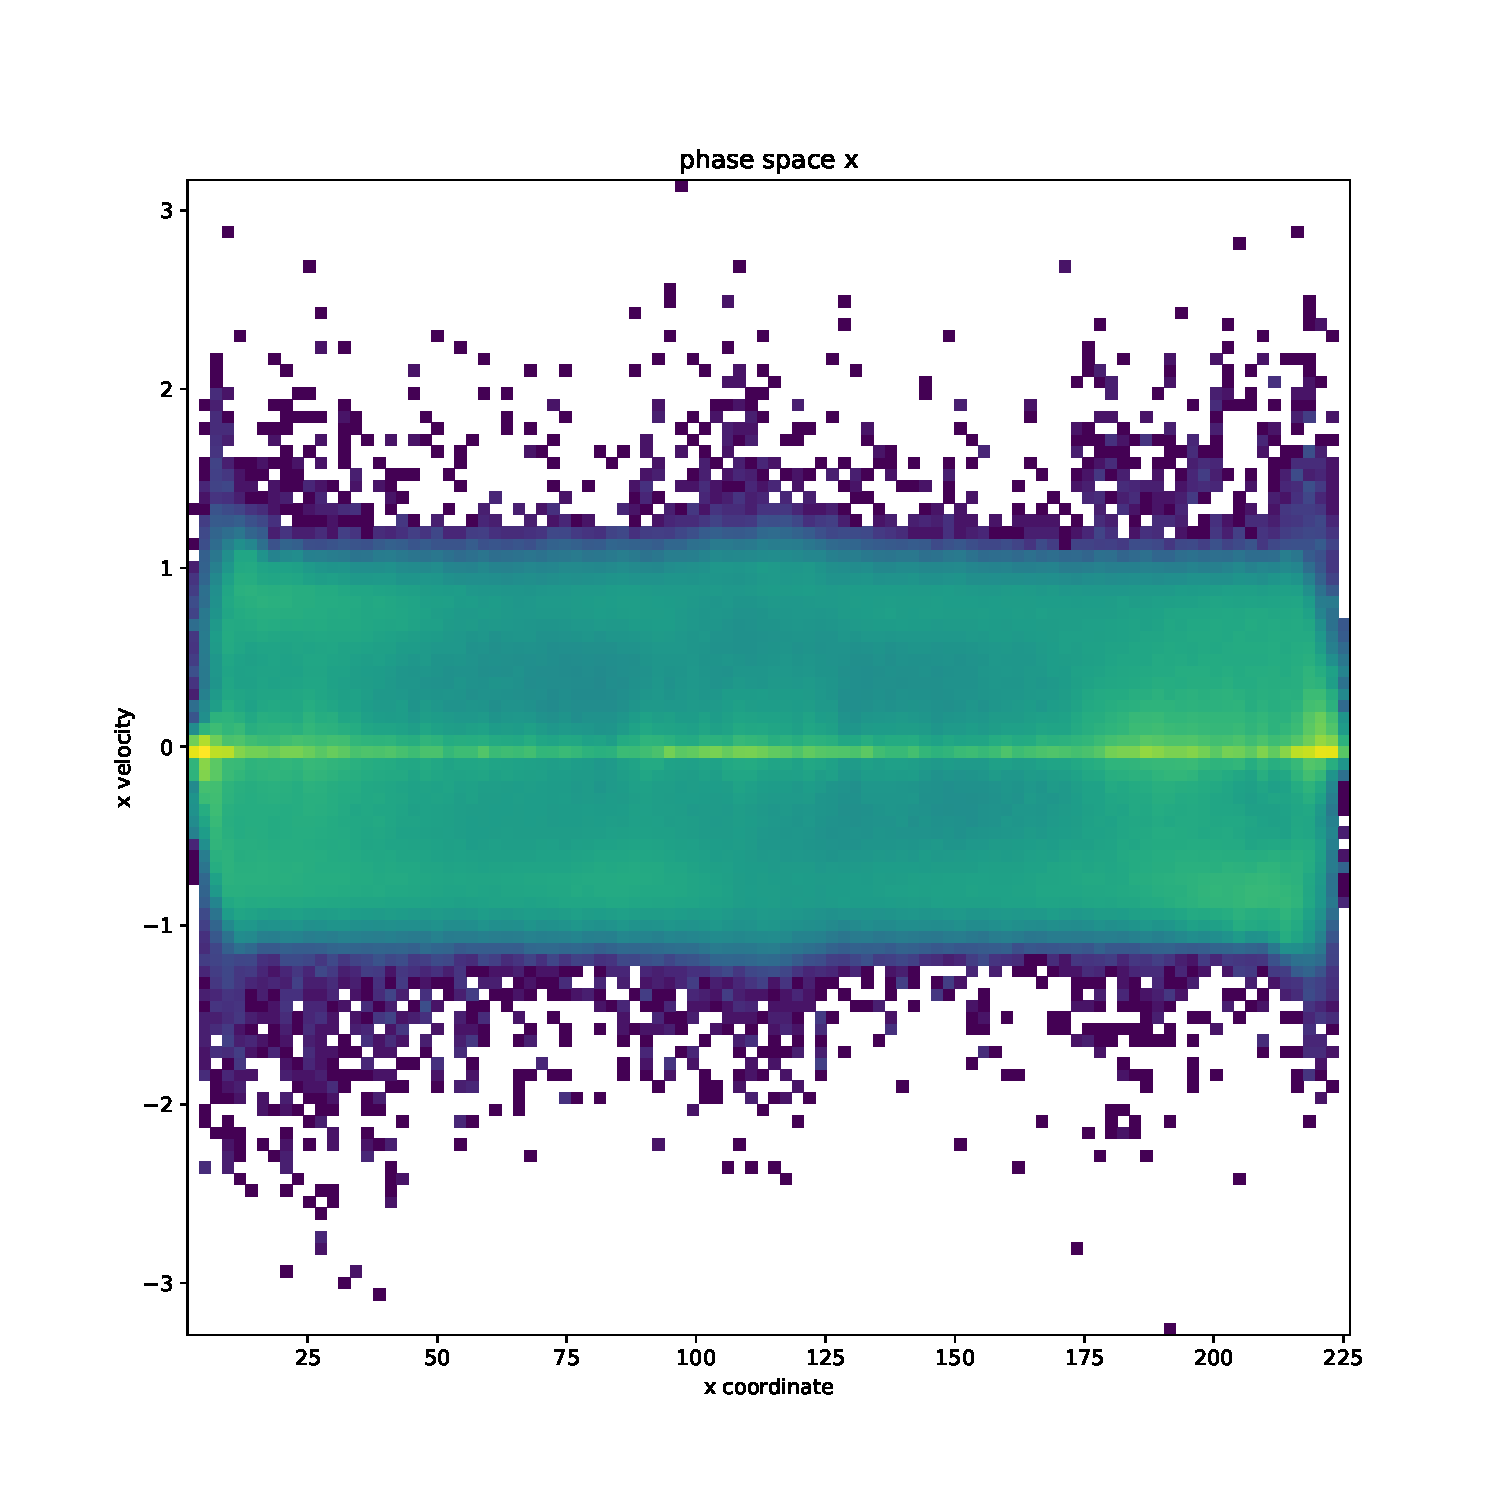
\includegraphics[ width=0.99\textwidth]{fig/hist2d_xvx/save_trainf10_pro_simTD2Q9Q9_hist2d_x_vx}
\captionsetup{width=0.9\linewidth}
\caption{\\Plot type (iii). \\Simulated dynamic using TD2Q9Q9}
\label{fig:xVx_SimTD2Q9Q9}
\end{minipage}
\end{figure}


% --- --- --- --- --- --- --- --- --- --- --- --- --- --- --- --- --- --- --- --- --- --- --- --- --- --- --- --- --- --- --- --- --- ---


\begin{figure}[ht]
\begin{minipage}[c]{1\linewidth}
\centering
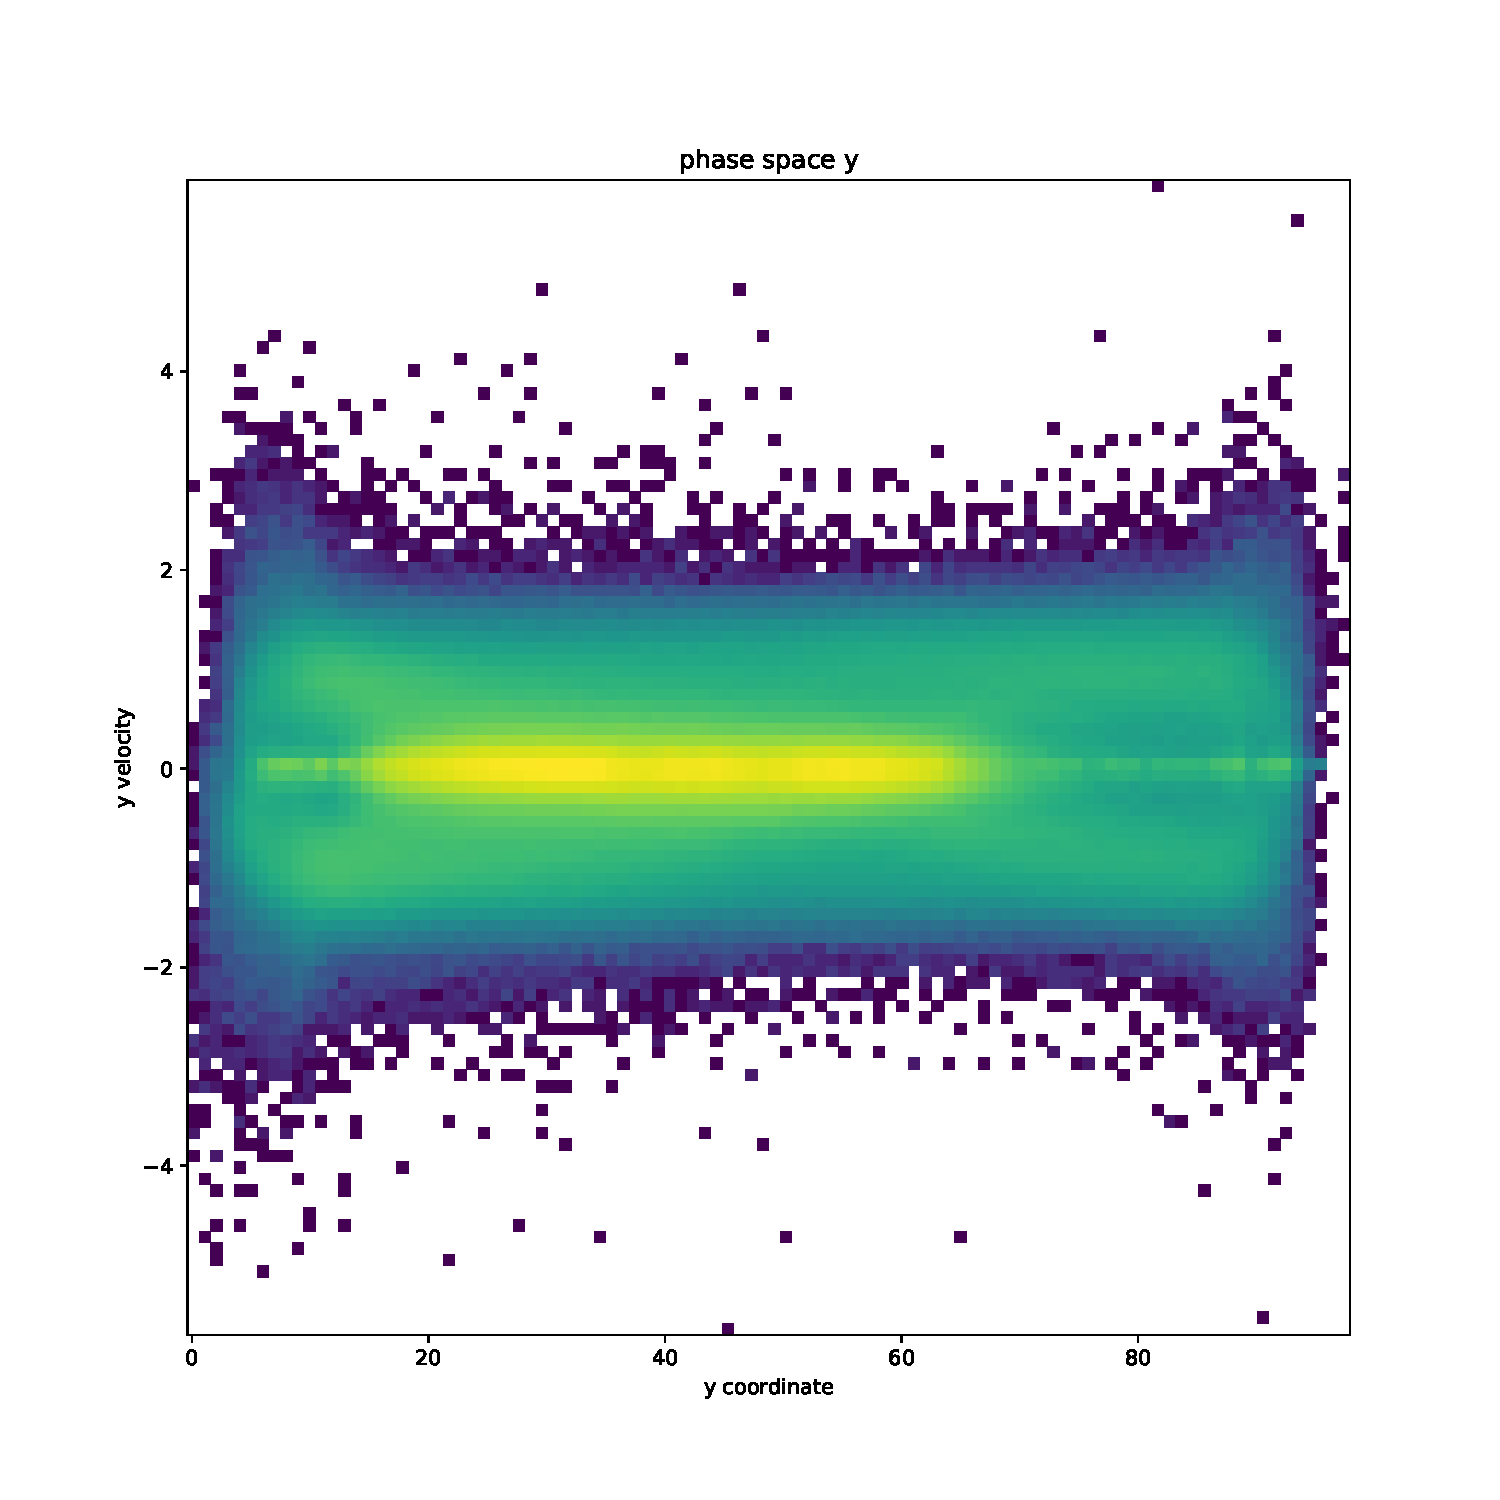
\includegraphics[ width=0.4\textwidth]{fig/hist2d_yvy/save_trainf10_pro_RealData_hist2d_y_vy}
\captionsetup{width=0.9\linewidth}
\caption{Plot type (iv). Real-life data distribution}
\label{fig:yVy_Real_iv}
\end{minipage}
\begin{minipage}[c]{0.24\linewidth}
\centering
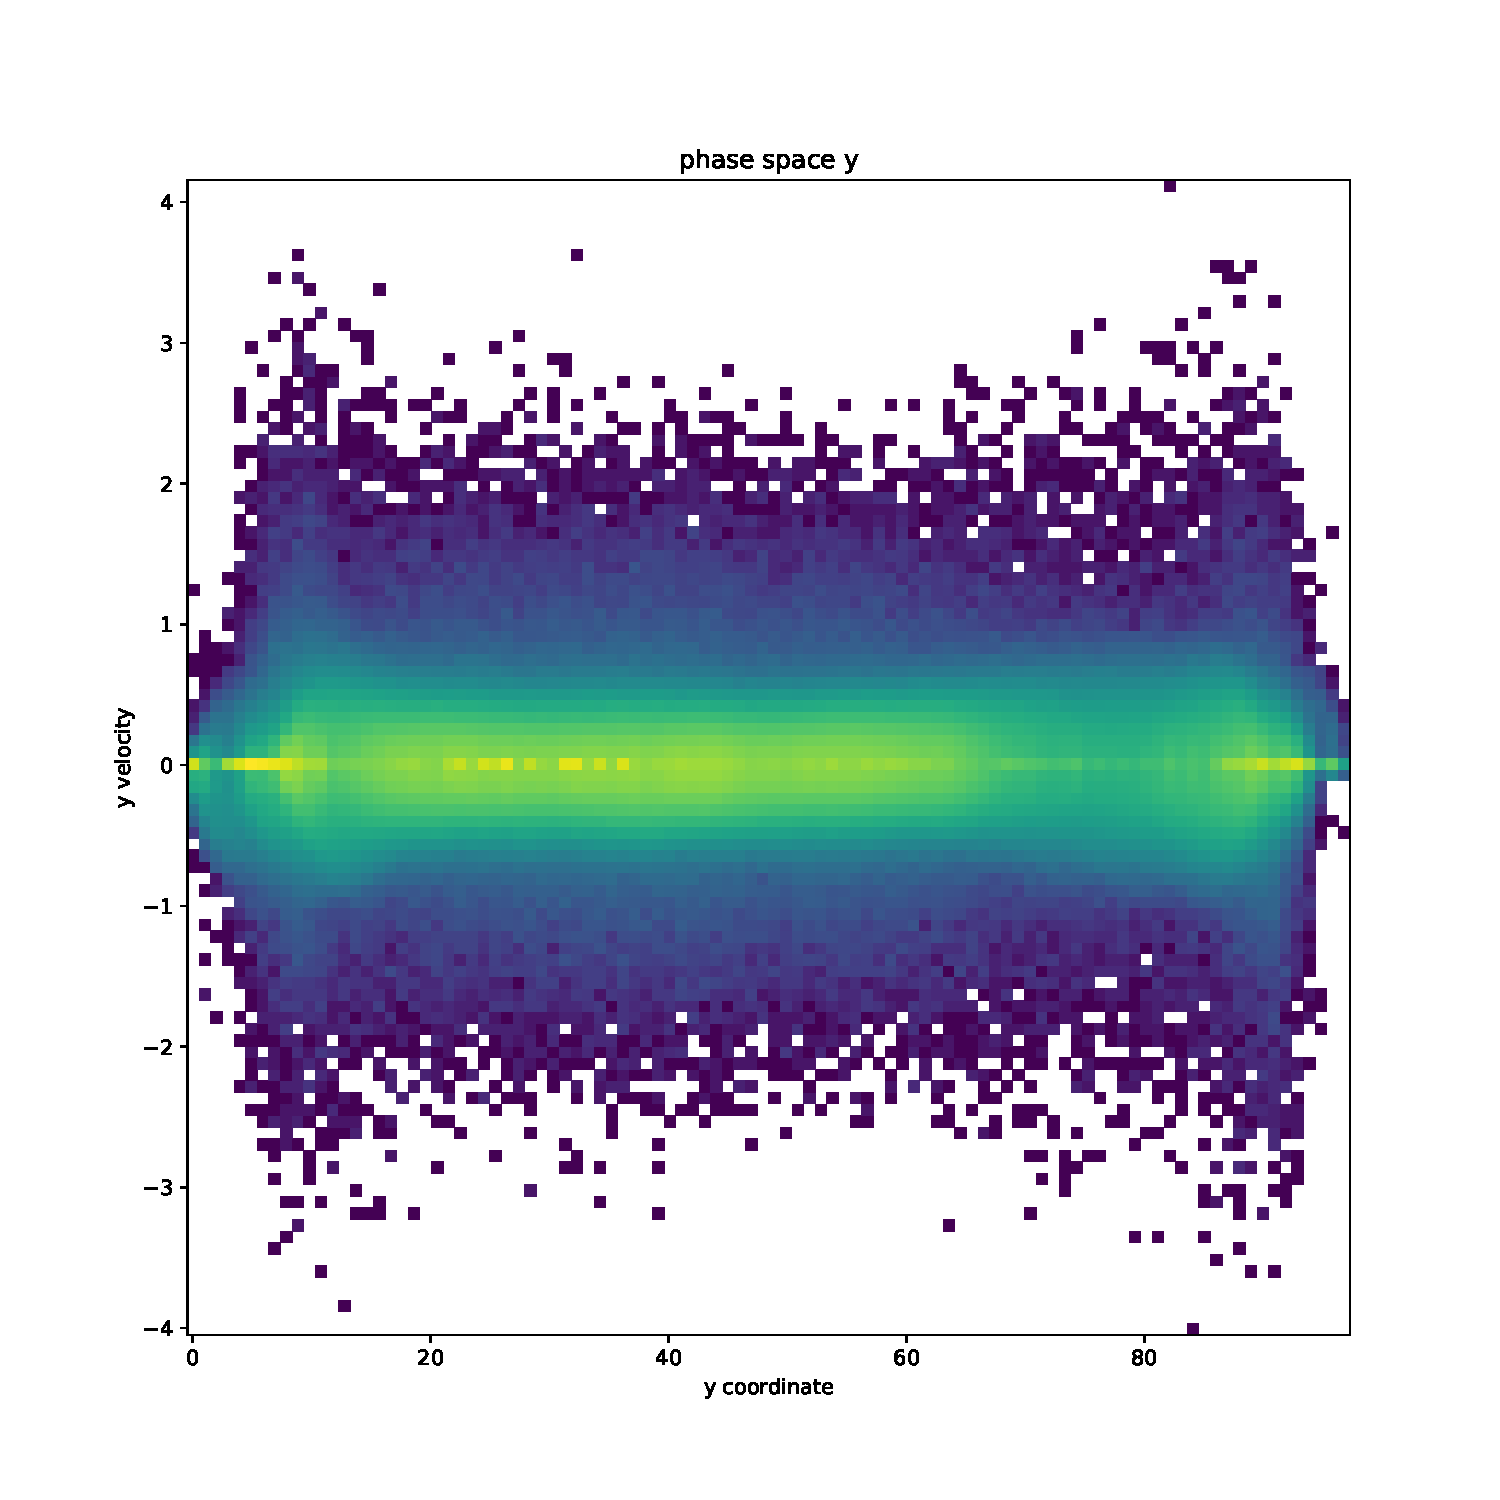
\includegraphics[ width=0.99\textwidth]{fig/hist2d_yvy/save_trainf10_pro_simD2Q9_hist2d_y_vy}
\captionsetup{width=0.9\linewidth}
\caption{\\Plot type (iv). \\Simulated dynamic using D2Q9}
\label{fig:yVy_SimD2Q9}
\end{minipage}
\begin{minipage}[c]{0.24\linewidth}
\centering
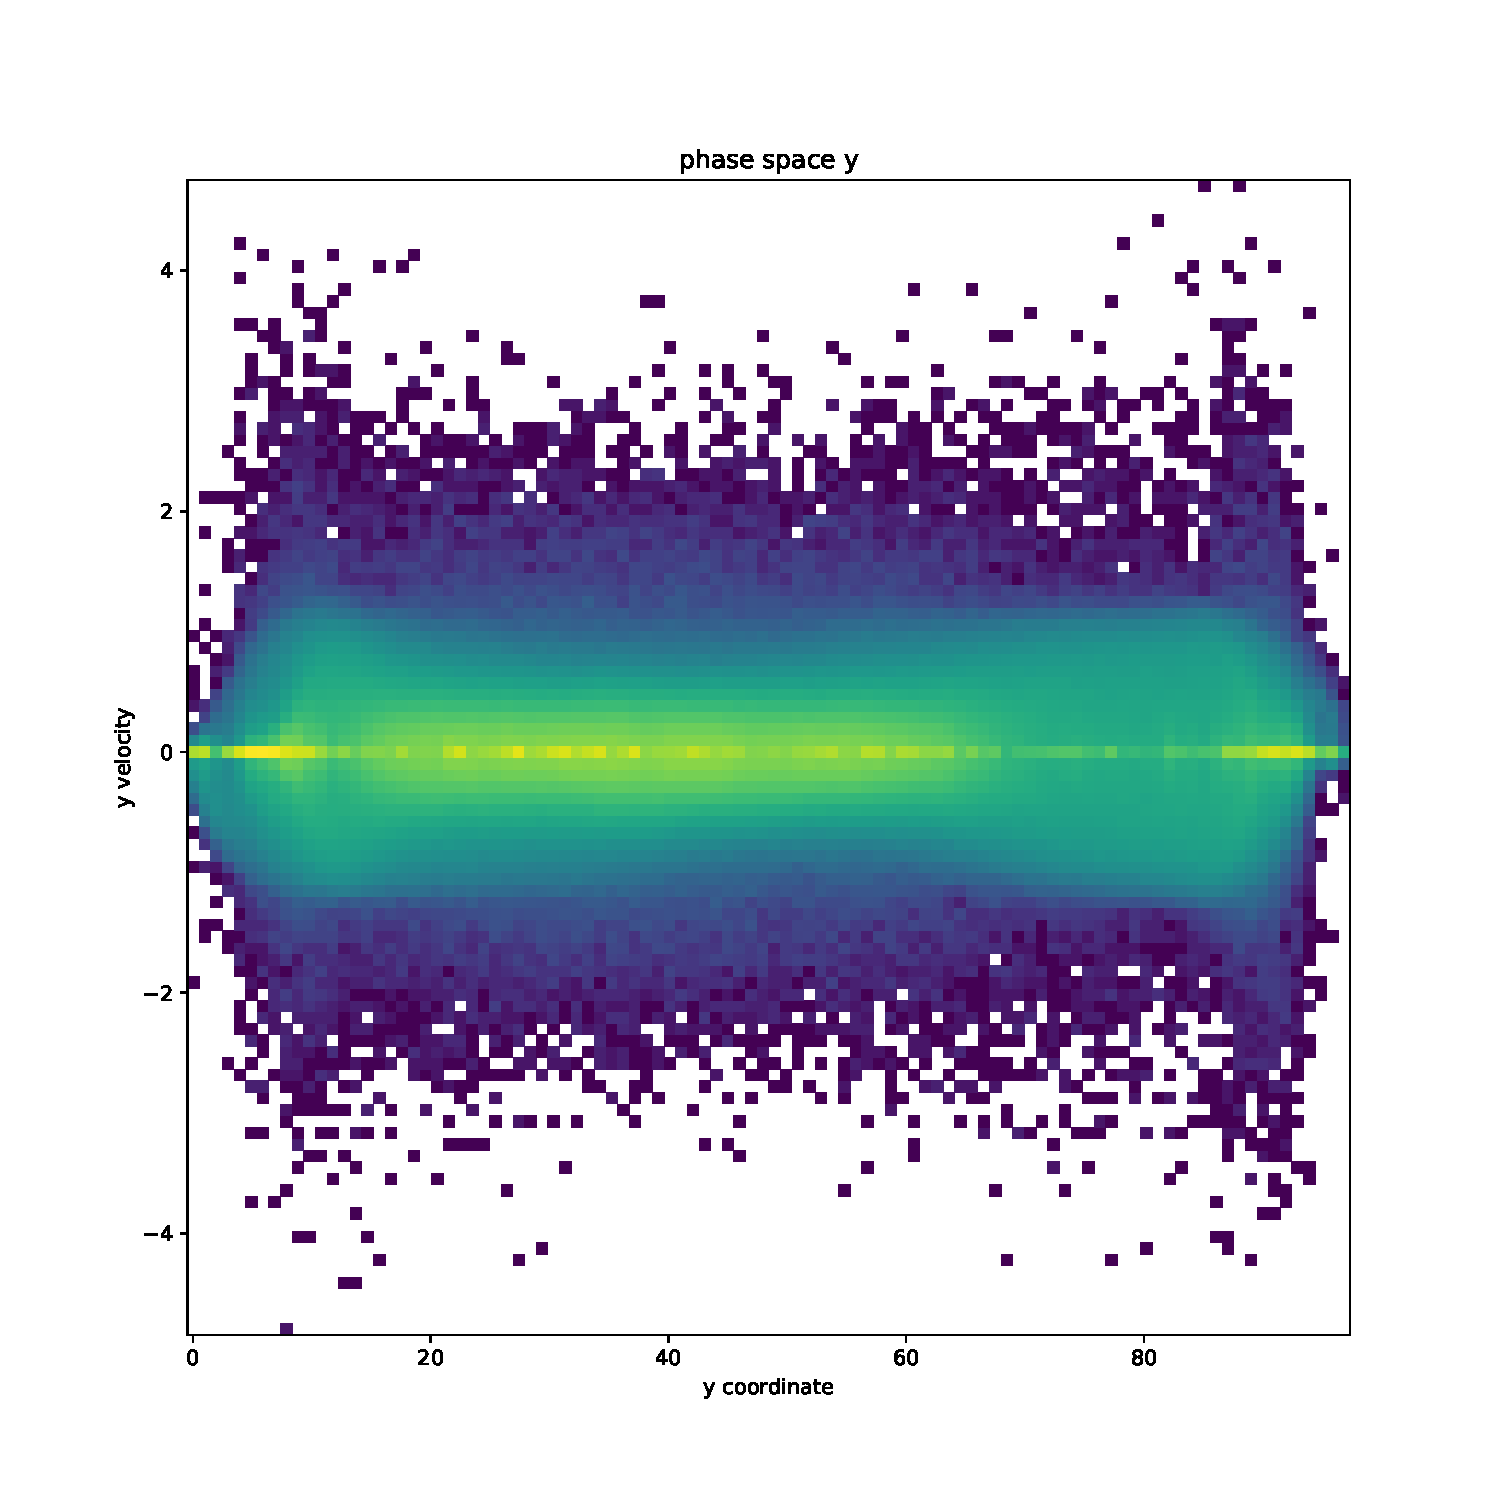
\includegraphics[ width=0.99\textwidth]{fig/hist2d_yvy/save_trainf10_pro_simD2Q9Q9_hist2d_y_vy}
\captionsetup{width=0.9\linewidth}
\caption{\\Plot type (iv). \\Simulated dynamic using D2Q9Q9}
\label{fig:yVy_SimD2Q9Q9}
\end{minipage}
\begin{minipage}[c]{0.24\linewidth}
\centering
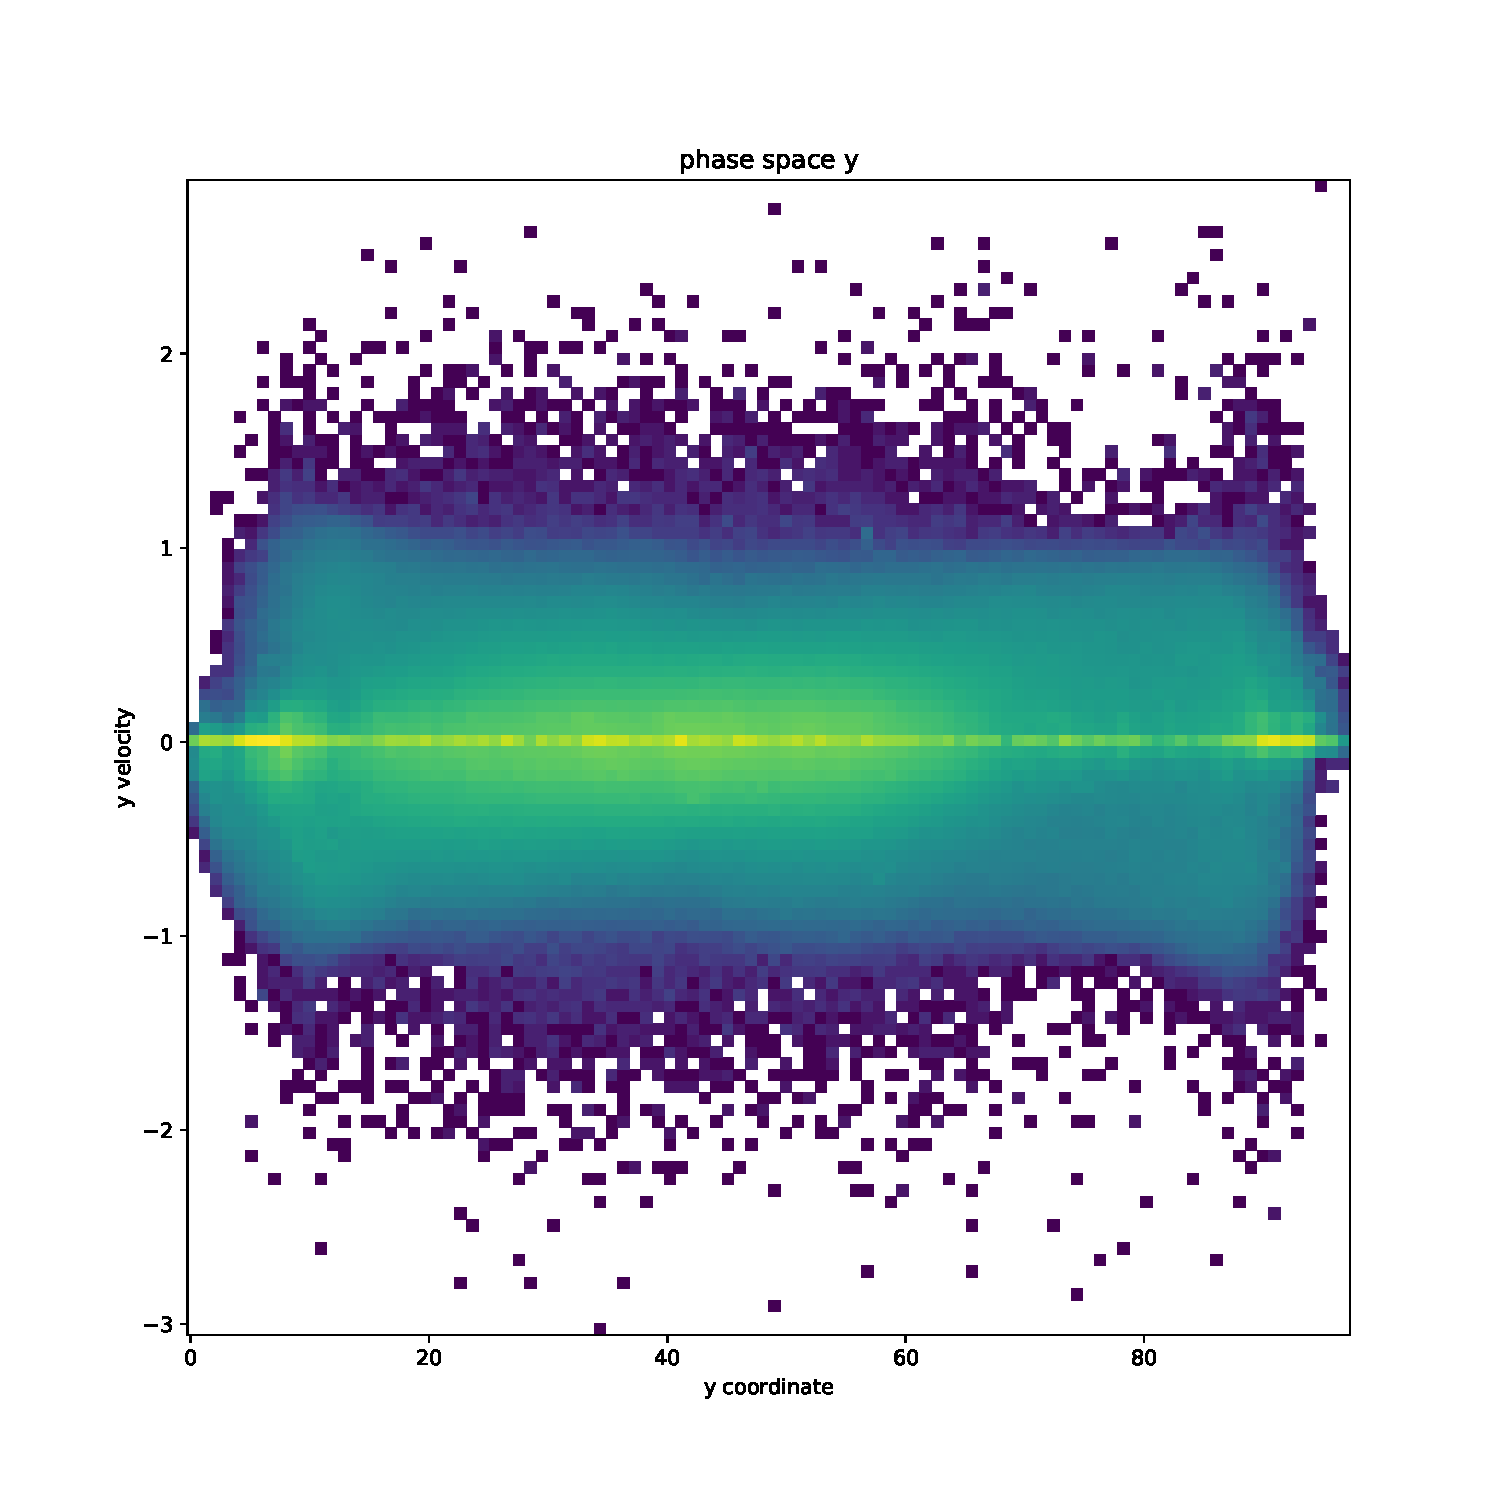
\includegraphics[ width=0.99\textwidth]{fig/hist2d_yvy/save_trainf10_pro_simTD2Q9_hist2d_y_vy}
\captionsetup{width=0.9\linewidth}
\caption{\\Plot type (iv). \\Simulated dynamic using TD2Q9}
\label{fig:yVy_SimTD2Q9}
\end{minipage}
\begin{minipage}[c]{0.24\linewidth}
\centering
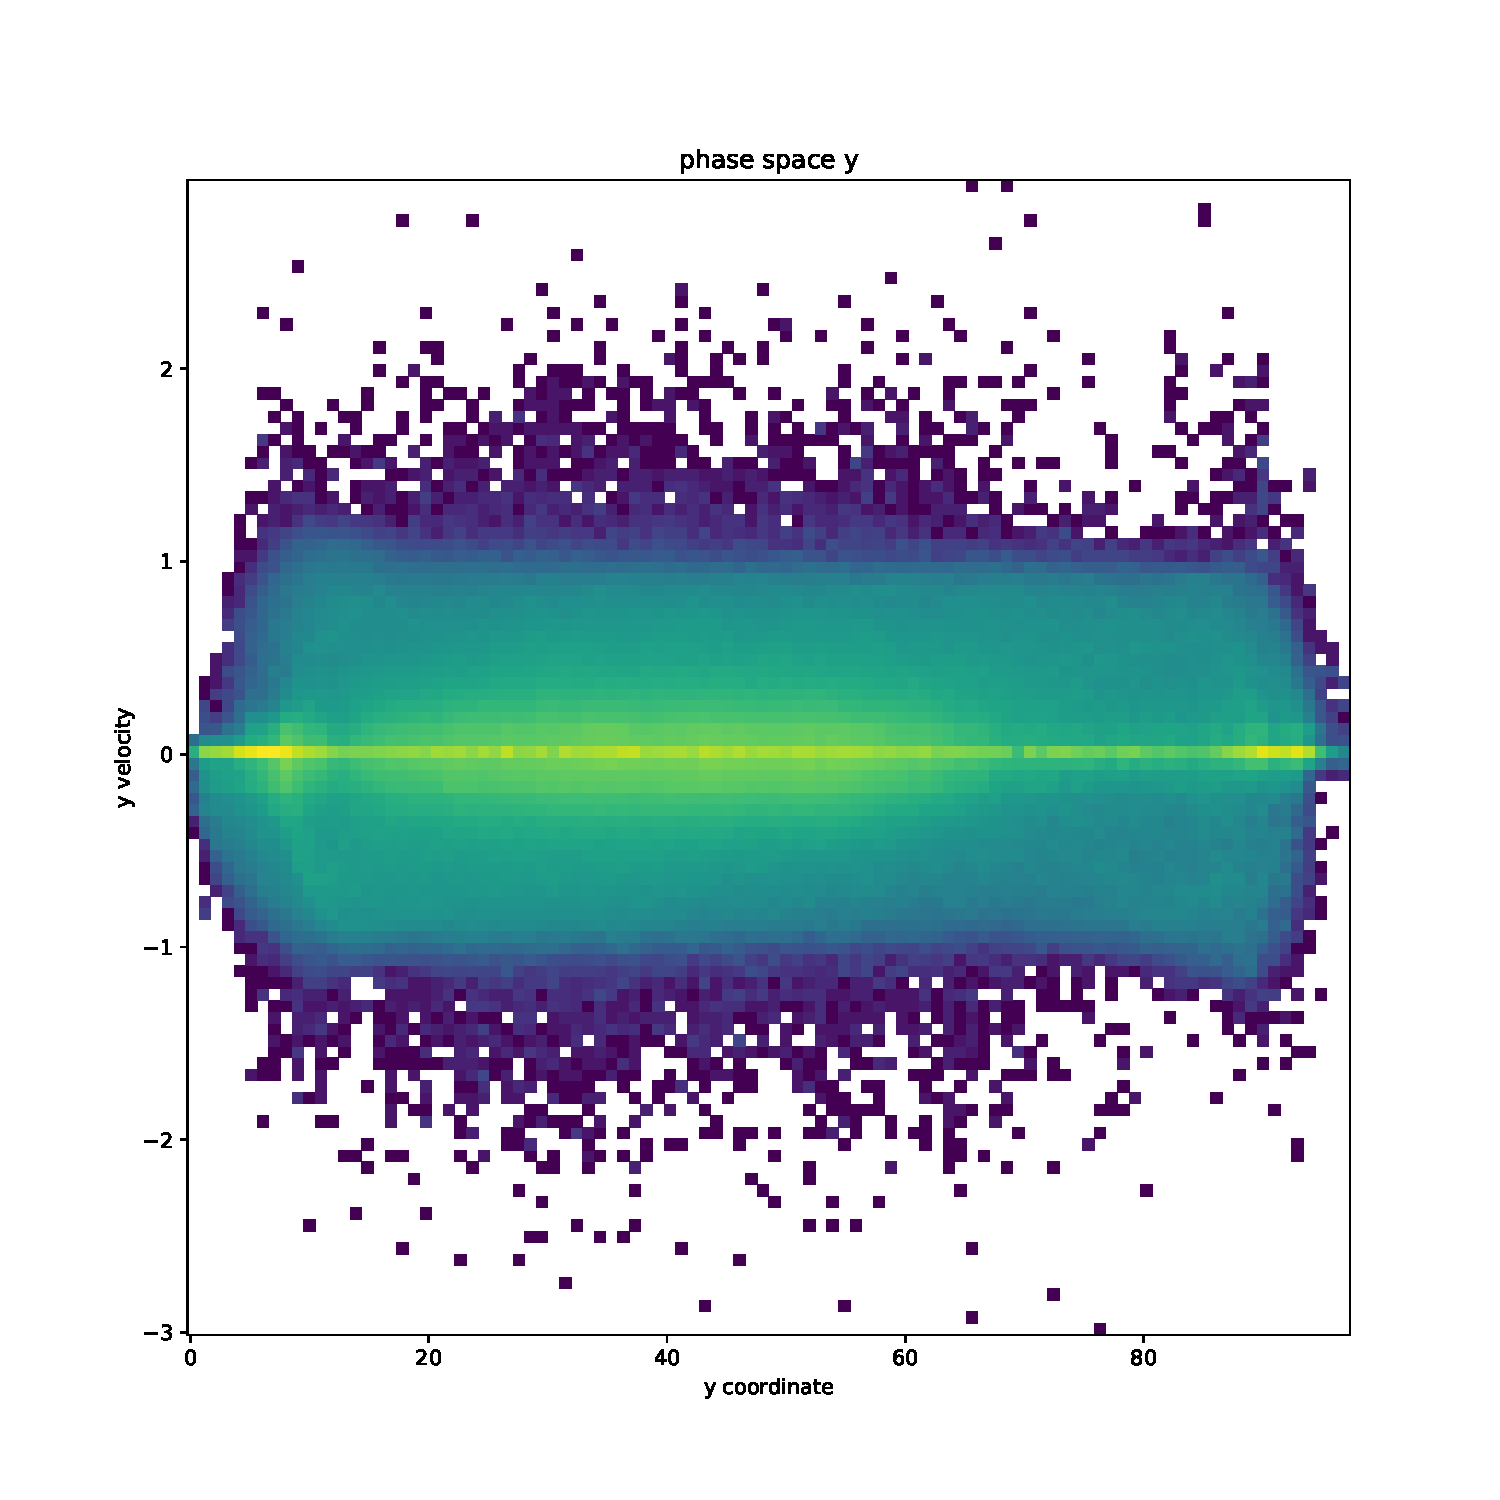
\includegraphics[ width=0.99\textwidth]{fig/hist2d_yvy/save_trainf10_pro_simTD2Q9Q9_hist2d_y_vy}
\captionsetup{width=0.9\linewidth}
\caption{\\Plot type (iv). \\Simulated dynamic using TD2Q9Q9}
\label{fig:yVy_SimTD2Q9Q9}
\end{minipage}
\end{figure}


% --- --- --- --- --- --- --- --- --- --- --- --- --- --- --- --- --- --- --- --- --- --- --- --- --- --- --- --- ---
\FloatBarrier
\newpage

The plots form (Figure \ref{fig:Pxy_Real_v}) to (Figure \ref{fig:Pxy_SimTD2Q9Q9}) represents the data about the (v) quantity.
\\ The first plot in (Figure \ref{fig:Pxy_Real_v}) shows where is more probable to find a pedestrian, in the considered field, based on real data.
The others from left to right represent the distribution of the position for every simulated datas.


\begin{figure}[ht]
\begin{minipage}[c]{1\linewidth}
\centering
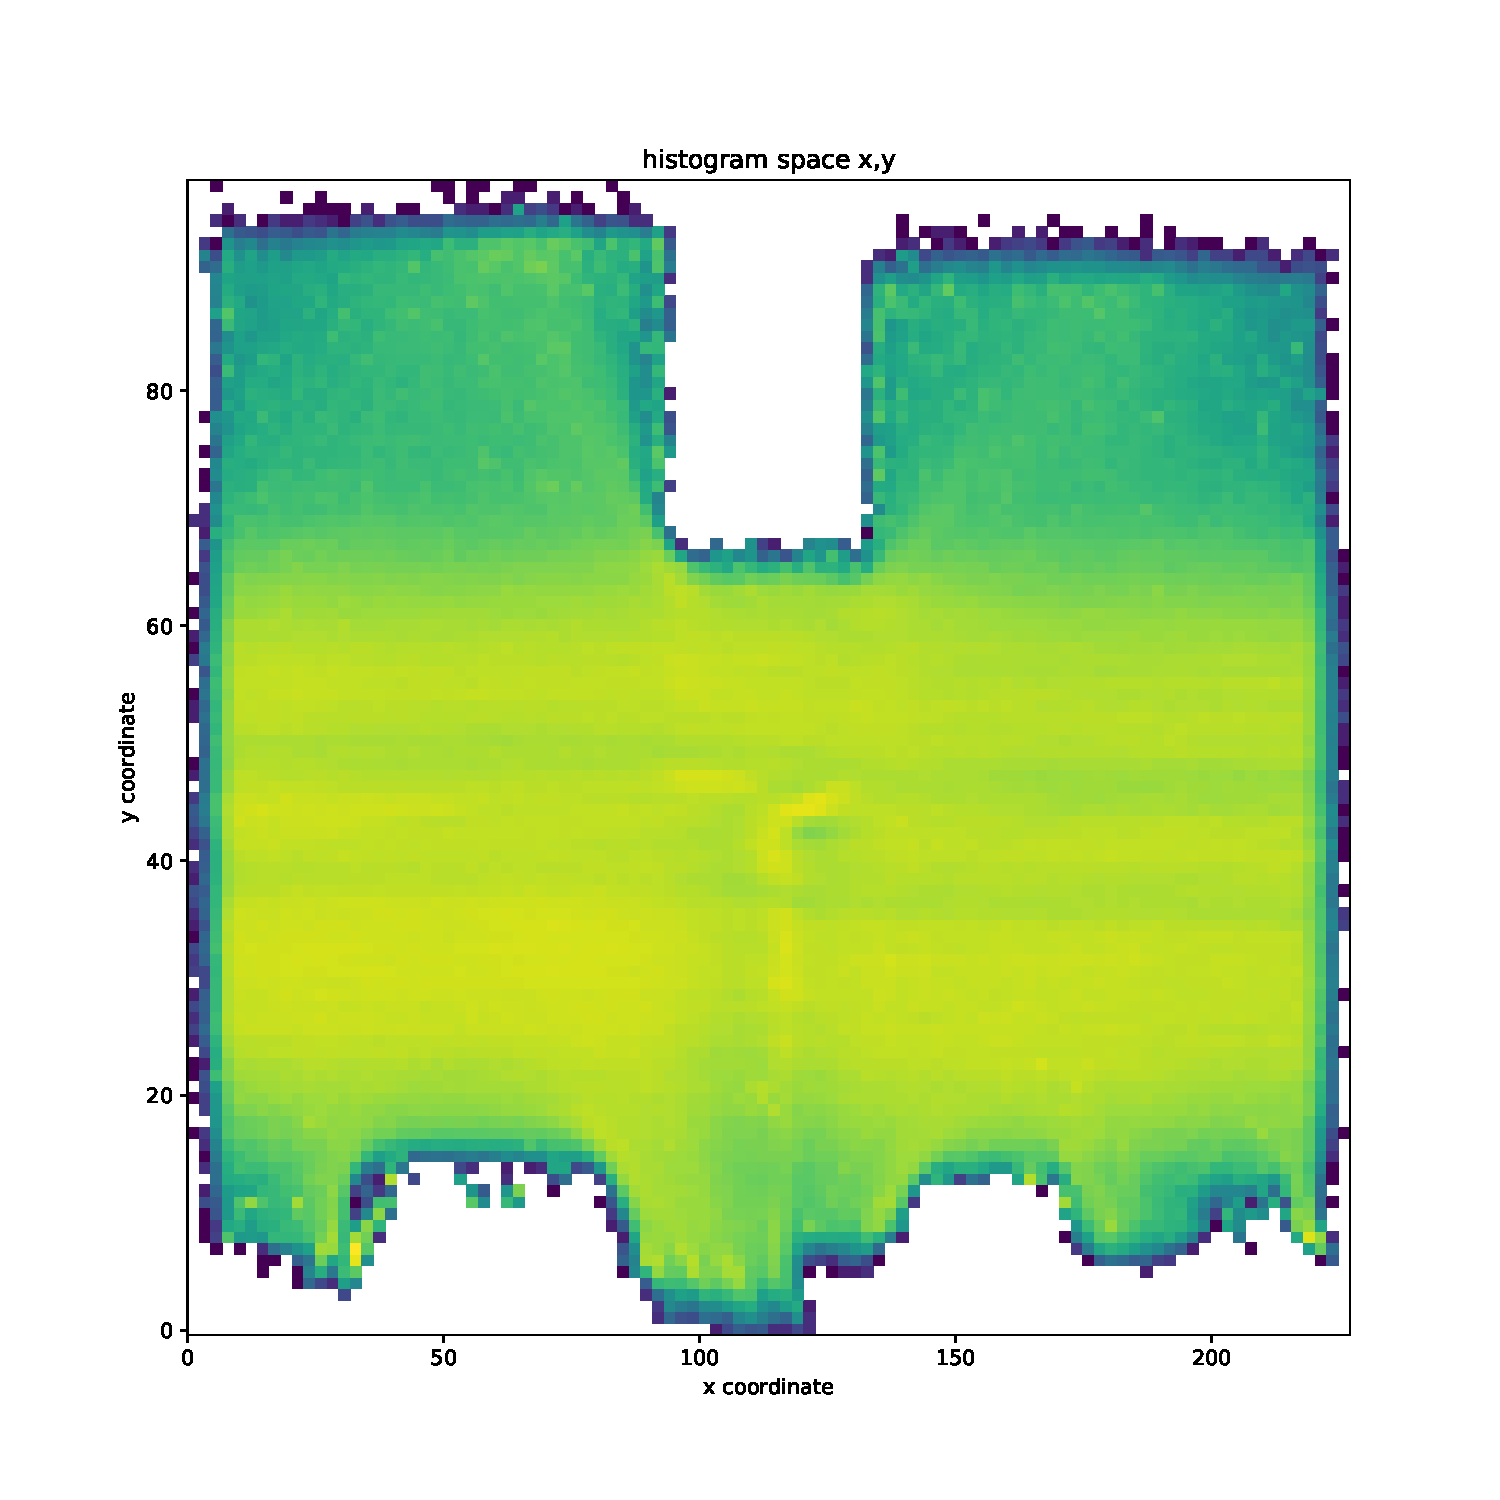
\includegraphics[ width=0.4\textwidth]{fig/hist2d_pxy/save_trainf10_pro_RealData_hist2d_x_y}
\captionsetup{width=0.9\linewidth}
\caption{Plot type (v). Real-life data distribution}
\label{fig:Pxy_Real_v}
\end{minipage}
\begin{minipage}[c]{0.24\linewidth}
\centering
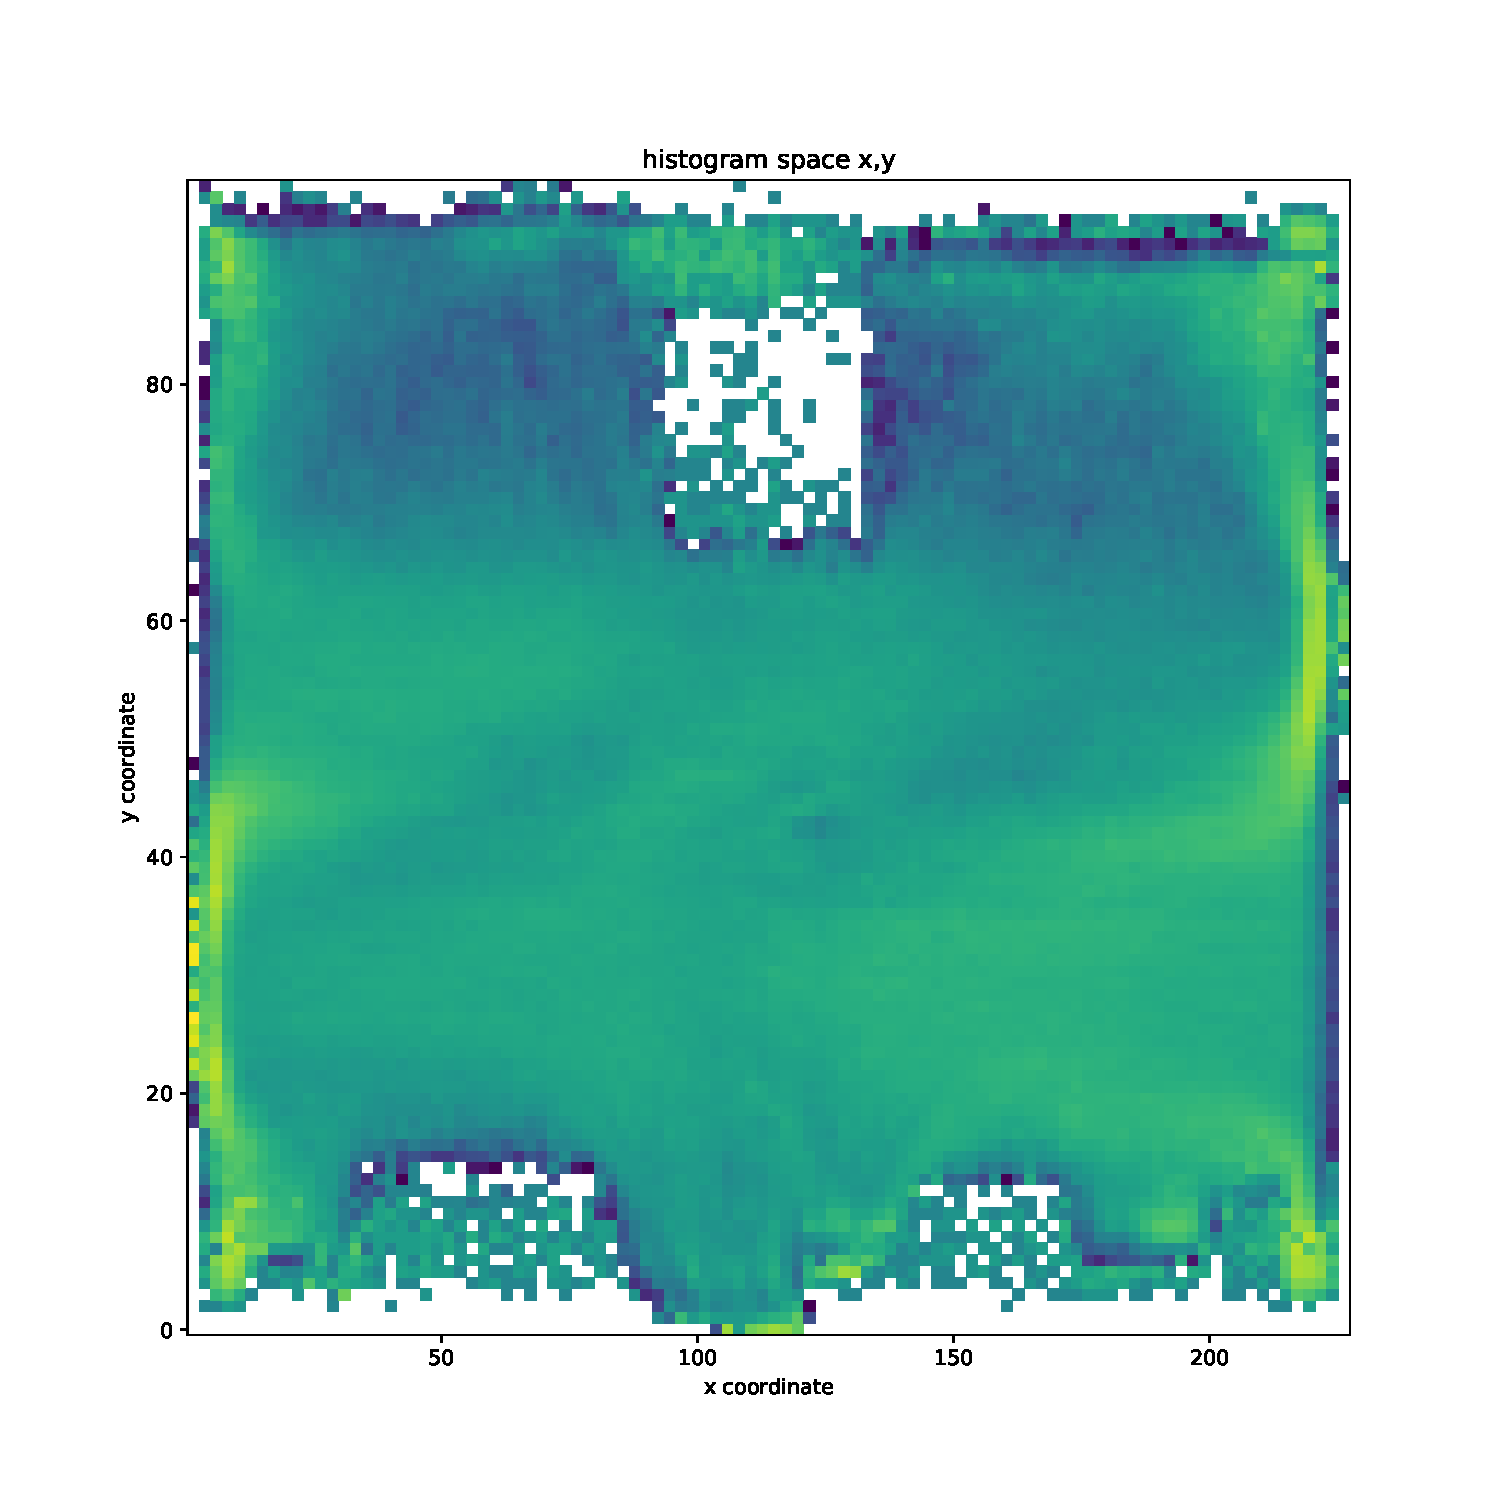
\includegraphics[ width=0.99\textwidth]{fig/hist2d_pxy/save_trainf10_pro_simD2Q9_hist2d_x_y}
\captionsetup{width=0.9\linewidth}
\caption{\\Plot type (v). \\Simulated dynamic using D2Q9}
\label{fig:Pxy_SimD2Q9}
\end{minipage}
\begin{minipage}[c]{0.24\linewidth}
\centering
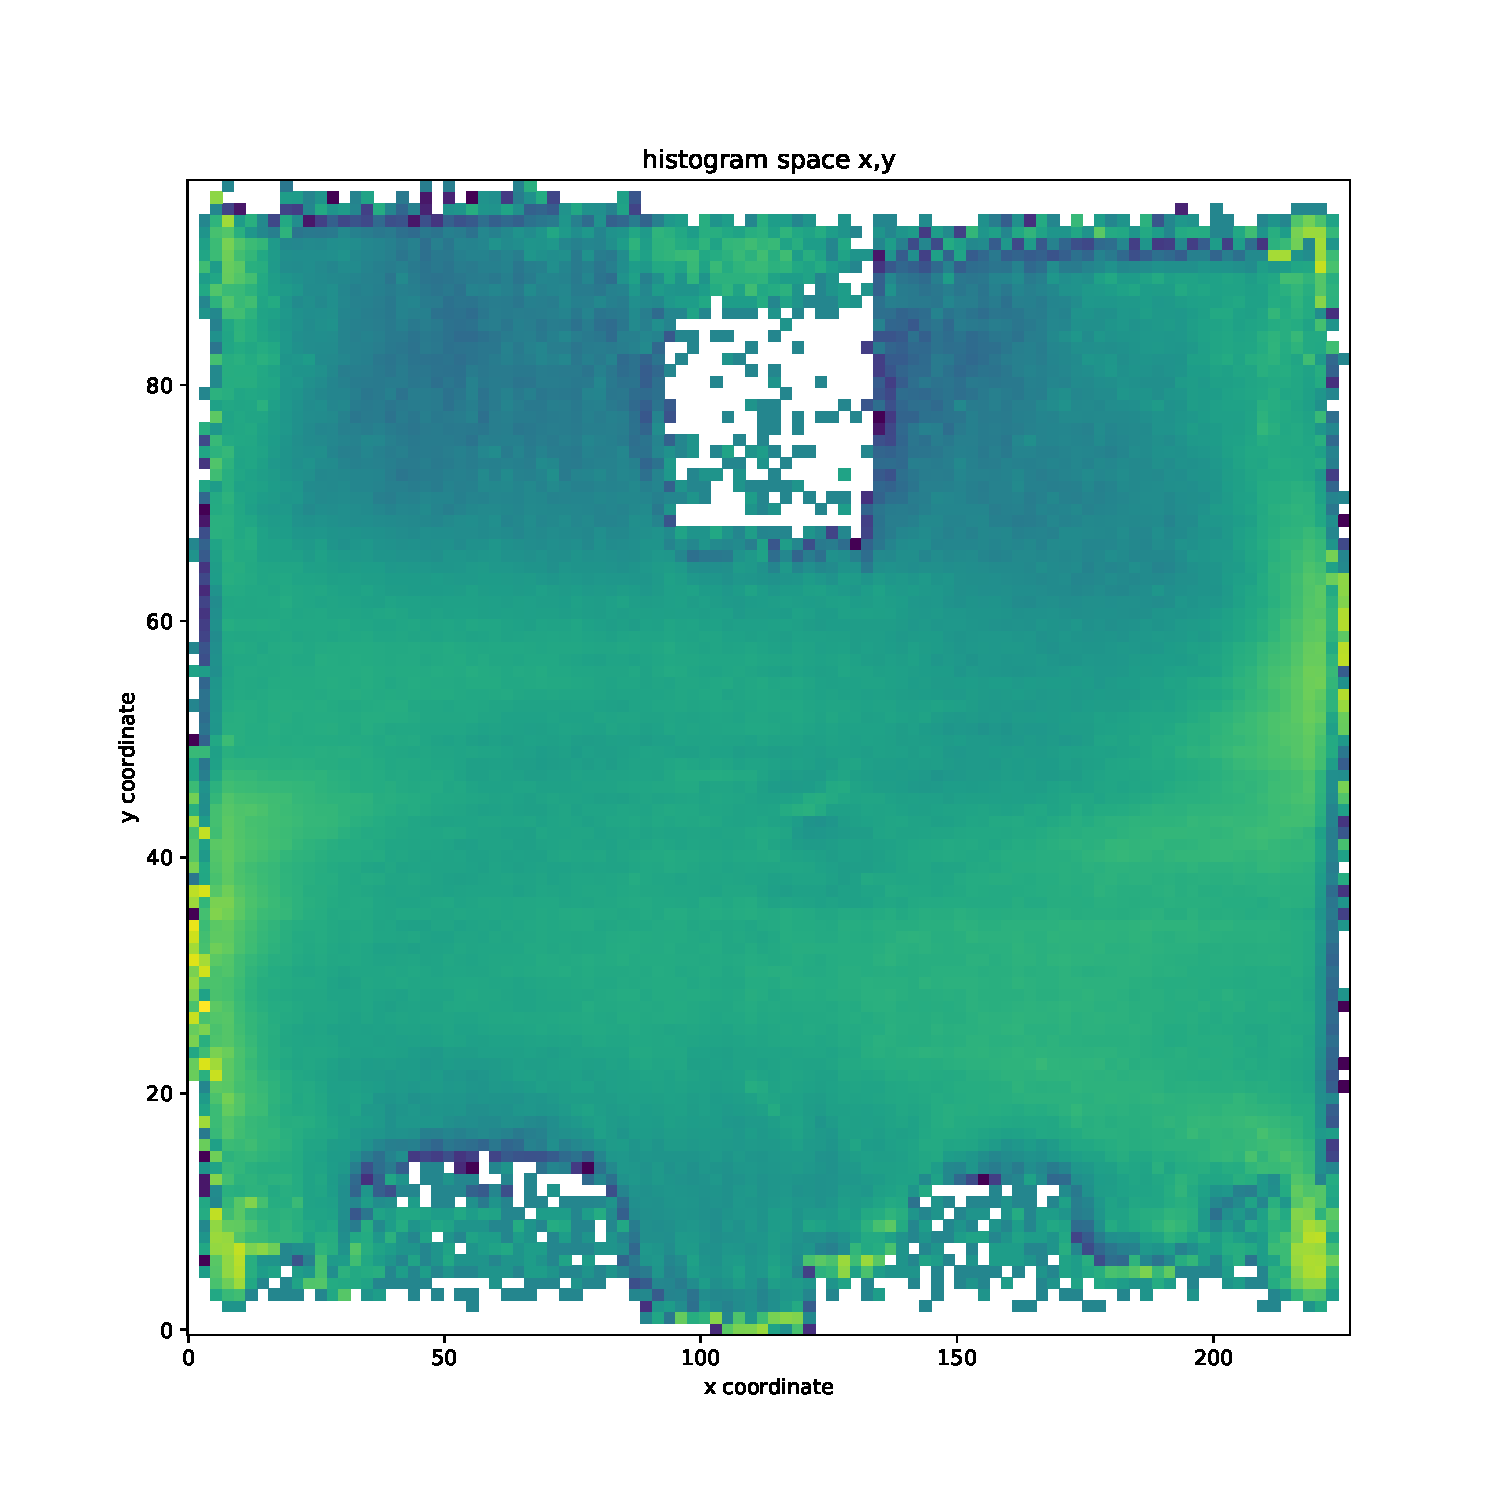
\includegraphics[ width=0.99\textwidth]{fig/hist2d_pxy/save_trainf10_pro_simD2Q9Q9_hist2d_x_y}
\captionsetup{width=0.9\linewidth}
\caption{\\Plot type (v). \\Simulated dynamic using D2Q9Q9}
\label{fig:Pxy_SimD2Q9Q9}
\end{minipage}
\begin{minipage}[c]{0.24\linewidth}
\centering
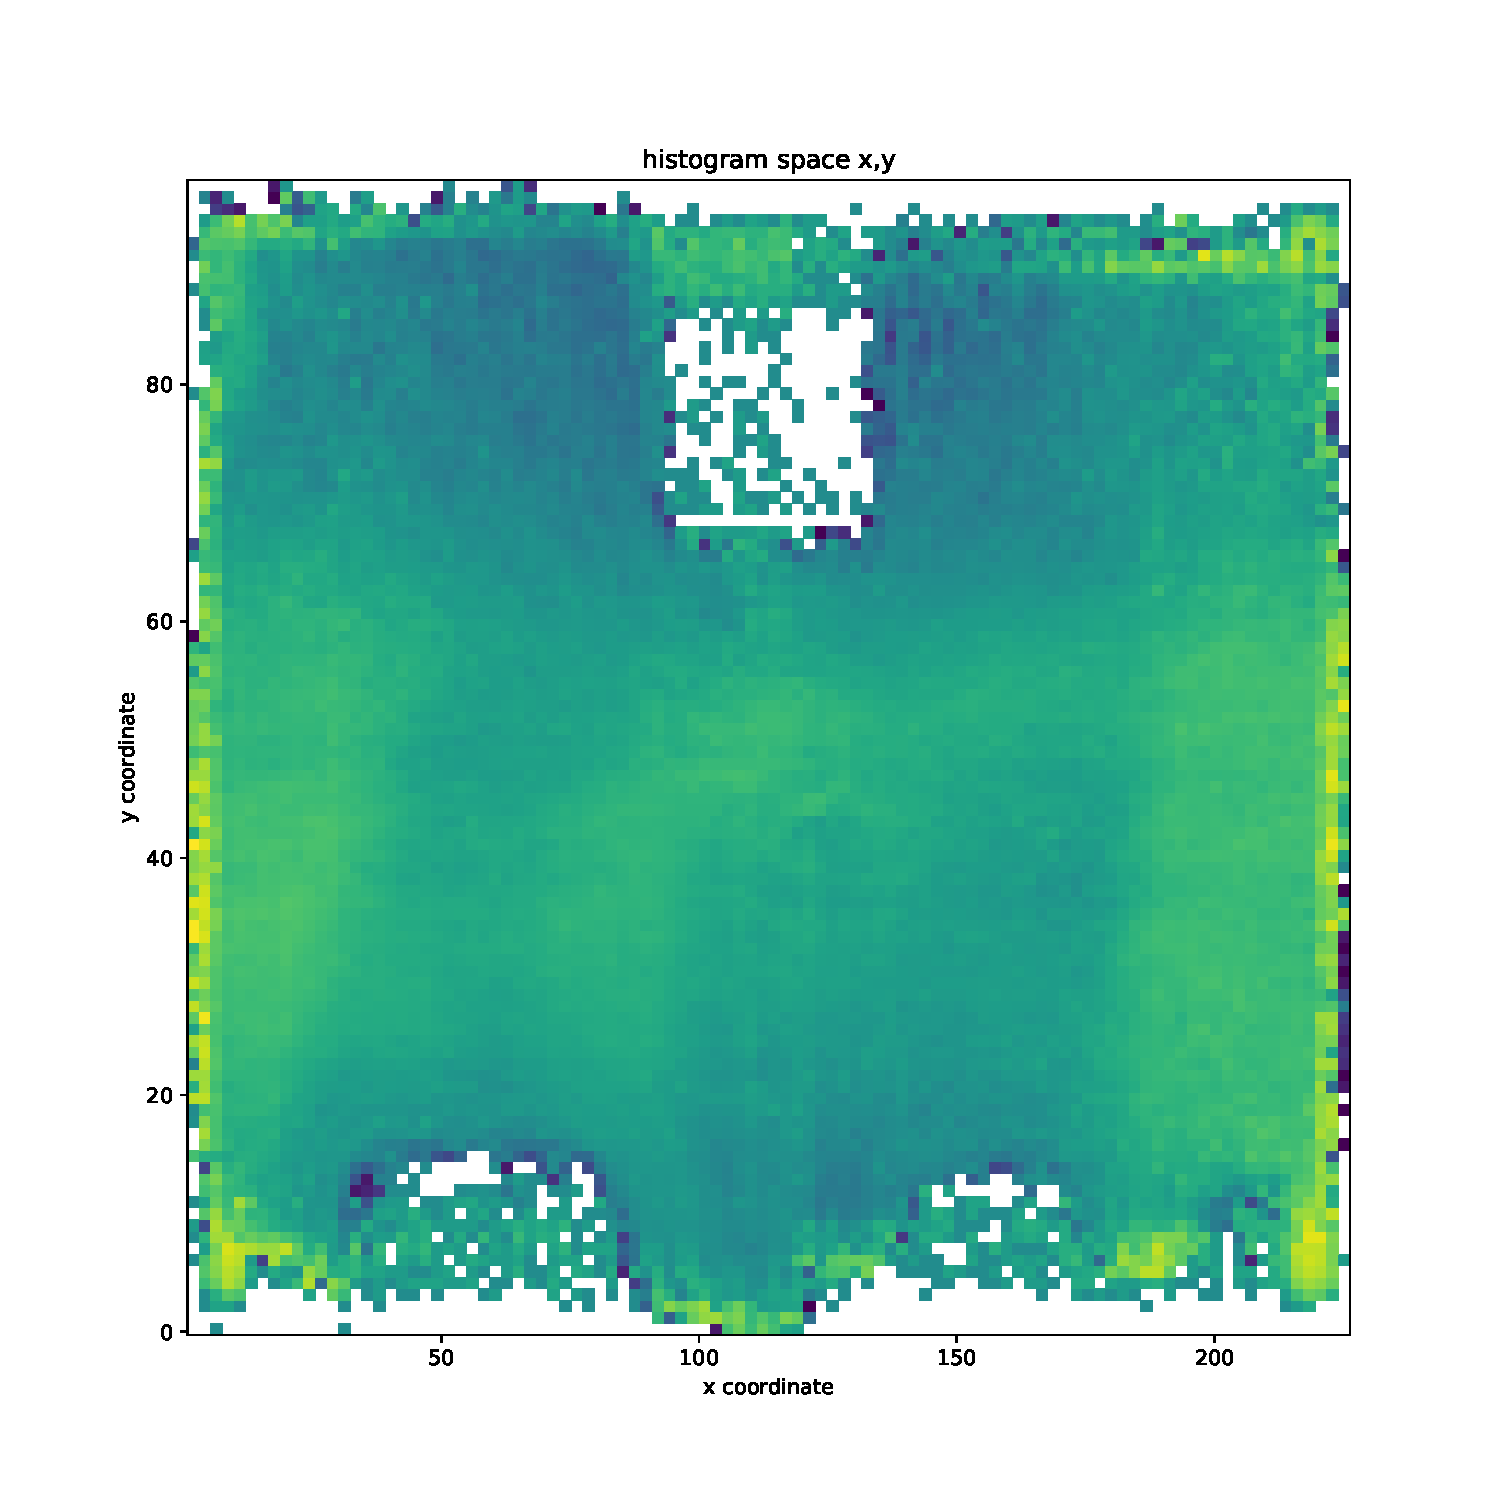
\includegraphics[ width=0.99\textwidth]{fig/hist2d_pxy/save_trainf10_pro_simTD2Q9_hist2d_x_y}
\captionsetup{width=0.9\linewidth}
\caption{\\Plot type (v). \\Simulated dynamic using TD2Q9}
\label{fig:Pxy_SimTD2Q9}
\end{minipage}
\begin{minipage}[c]{0.24\linewidth}
\centering
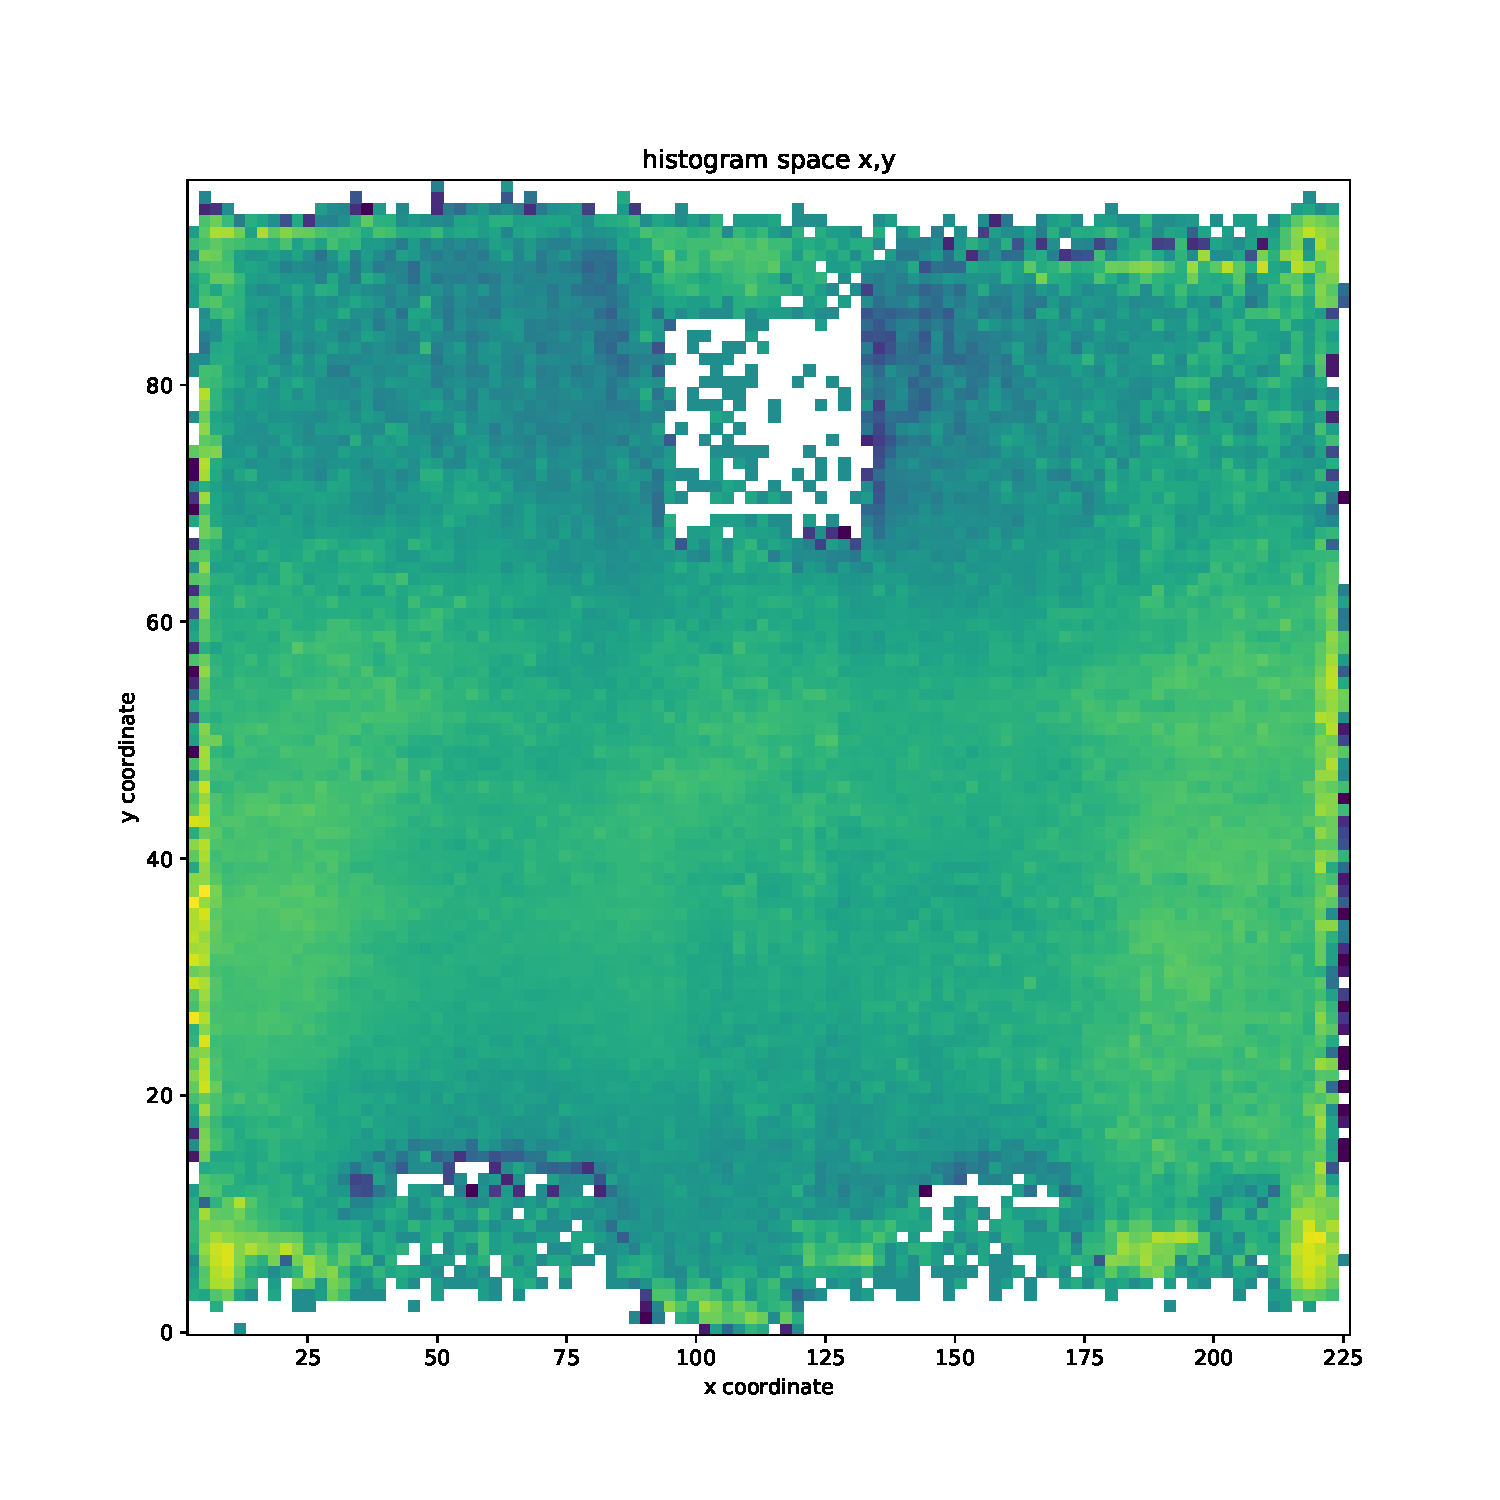
\includegraphics[ width=0.99\textwidth]{fig/hist2d_pxy/save_trainf10_pro_simTD2Q9Q9_hist2d_x_y}
\captionsetup{width=0.9\linewidth}
\caption{\\Plot type (v). \\Simulated dynamic using TD2Q9Q9}
\label{fig:Pxy_SimTD2Q9Q9}
\end{minipage}
\end{figure}


% --- --- --- --- --- --- --- --- --- --- --- --- --- --- --- --- --- --- --- --- --- --- --- --- --- --- --- --- ---
\FloatBarrier
In this study case there is a strong $x$ component in the pedestrian's motion.
A great number of trajectories go through the space from left to right or vice-versa with a \emph{quasi}-straight horizontal path.
A minor number of pedestrians make they way going from up to down or vice-versa through the filed with a \emph{quasi}-straight vertical line.
Some others trajectories make a visible change in direction, e.g. from going straight horizontal to right-up when exiting the area.
This dataset has a \emph{good} variety of cases, that sufficiently represents how pedestrians may move along the field.
With this it's possible to generate synthetic pedestrian made by simulating theirs dynamic, entirely based on real observation.






\FloatBarrier
\end{document}
